%% LyX 2.4.0 created this file.  For more info, see https://www.lyx.org/.
%% Do not edit unless you really know what you are doing.
\documentclass[11pt,english]{article}
\usepackage{lmodern}
\renewcommand{\familydefault}{\rmdefault}
\usepackage[T1]{fontenc}
\usepackage[latin9]{inputenc}
\usepackage{geometry}
\geometry{verbose,tmargin=1in,bmargin=1in,lmargin=1in,rmargin=1in}
\usepackage{babel}
\usepackage{amstext}
\usepackage{graphicx}
\usepackage{setspace}
\usepackage[authoryear]{natbib}
\onehalfspacing
\usepackage[pdfusetitle,
 bookmarks=true,bookmarksnumbered=false,bookmarksopen=false,
 breaklinks=false,pdfborder={0 0 0},pdfborderstyle={},backref=false,colorlinks=false]
 {hyperref}

\makeatletter
%%%%%%%%%%%%%%%%%%%%%%%%%%%%%% User specified LaTeX commands.
\date{}
% Added by lyx2lyx
\setlength{\parskip}{\medskipamount}
\setlength{\parindent}{0pt}

\ifdefined\showcaptionsetup
 % Caption package is used. Advise subfig not to load it again.
 \PassOptionsToPackage{caption=false}{subfig}
\fi
\usepackage{subfig}
\makeatother

\begin{document}
\title{Poverty Mapping in the Age of Machine Learning\thanks{The authors acknowledge financial support from the World Bank. We
thank Roy van der Weide and Isabel Molina for comments. Additionally,
we thank Benu Bidani, Carlos Rodriguez-Castelan, and Johan Mistiaen
for providing support and space to pursue this work. Finally, we thank
the Global Solutions Group on Data for Policy. Any error or omission
is the authors\textquoteright{} responsibility alone.}}
\author{Paul Corral,\thanks{The World Bank Group - Poverty and Equity Global Practice (pcorralrodas@worldbank.org)}
Heath Henderson,\thanks{Department of Economics and Finance, Drake University, United States
of America} and Sandra Segovia\thanks{The World Bank Group - Poverty and Equity Global Practice} }
\maketitle
\begin{abstract}
Recent years have witnessed considerable methodological advances in
poverty mapping, much of which has focused on the application of modern
machine-learning approaches to remotely-sensed data. Poverty maps
produced with these methods generally share a common validation procedure,
which assesses model performance by comparing sub-national poverty
estimates with survey-based, direct estimates. While unbiased, direct
estimates can be imprecise measures of true poverty rates, meaning
that it is unclear whether the standard validation procedures are
informative of actual model performance. In this paper, we examine
the credibility of existing approaches to model validation by constructing
a pseudo-census from the Mexican Intercensal Survey of 2015, which
we use to conduct several simulation experiments. We find that the
standard validation procedure can be misleading in terms of model
assessment, with notable implications for model selection. Further,
we find that our closest approximation to existing machine-learning
approaches performs poorly when evaluated against ``true'' poverty
rates and fails to outperform traditional poverty mapping methods
in targeting simulations.

\vfill{}
\end{abstract}
\textbf{Key words:} Small area estimation; poverty mapping; machine
learning; satellite imagery 

\textbf{JEL classification: }C13; C55; C87; C15\pagebreak{}

\section{Introduction}

Poverty maps provide granular estimates of poverty at the sub-national
level in order to better inform the targeting of resources and support
the design of interventions tailored to local needs (\citealt{bedi2007more,elbers2007poverty}).
As household surveys are generally unrepresentative for small geographical
areas, producing detailed poverty maps often requires using small
area estimation, which consists of using statistical methods to predict
poverty levels on the basis of household- or area-level characteristics.
The basic procedure entails two steps: (1) using household survey
data, fit a statistical model at the household or area level of some
welfare measure (e.g., poverty, income, or wealth) to household- or
area-level characteristics, and (2) apply the model to census data
available for all households or geographical entities to estimate
poverty at the sub-national level. At a minimum, the procedure thus
requires a household survey and data at the area level or a census
to produce a sufficiently detailed poverty map.

The literature on small area estimation is rich and several variations
on this basic procedure have been proposed. Unit-level models conduct
estimation and prediction at the household level, assuming a linear
relationship between the welfare measure and covariates \citep{hentschel1998combining,elbers2003micro,molina2010small}.
Unit-level models are not well-suited to situations where the survey
and census data correspond to different years, which is often the
case in developing countries where censuses are conducted infrequently.
Area-level models represent a feasible alternative for periods where
a recent census is not available that similarly relies on linear functional
forms, but conduct estimation and prediction using only aggregate
data for the geographical entities of interest \citep{fay1979estimates,torabi2014small}.
Unit-context models have been suggested alternative and are characterized
by an estimation stage wherein household-level measures are modeled
exclusively as a linear function of area-level characteristics \citep{nguyen2012method,lange2018small,masaki2020small}.

Recent developments in poverty mapping have focused on the application
of machine learning to remotely-sensed data, largely in response to
the issue of out-of-date census information. These approaches also
use survey-derived welfare measures, but are distinguished by a first
stage where a machine-learning model is fit to remotely-sensed covariates
(e.g., data derived from satellite imagery or call detail records)
rather than census-based covariates. For example, \citet{chi2022microestimates}
matched data from several remotely-sensed data sources to survey-based
measures of ``village'' wealth for 56 countries, and then fit a
prediction model using gradient boosting machines.\footnote{Their remotely-sensed data includes high-resolution satellite imagery,
mobile phone data, topographic maps, and connectivity data from Facebook.} They then applied the model to the populated surface of all 135 low-
and middle-income countries to develop granular poverty maps for each
country. Similar approaches have been used for individual countries,
including Rwanda \citep{blumenstock2015predicting}, Senegal \citep{pokhriyal2017combining},
Bangladesh \citep{steele2017mapping}, and Belize \citep{hersh2021open},
among others.\footnote{See \citet{jean2016combining}, \citet{yeh2020using}, \citet{lee2020high},
and \citet{aiken2022machine} for examples of other recent applications.}

While often subsumed under the term ``machine learning,'' this modern
approach to poverty mapping actually consists of several practices
that differ from more traditional approaches. Most obviously, the
modern approach substitutes non-parametric statistical methods for
the parametric approaches traditionally used for poverty mapping.
In addition, the modern approach relies heavily on remotely-sensed
covariates rather than covariates derived from census data.\footnote{Nevertheless, traditional area-level metods have made considerable
use of remotely sensed covariates and often rely on using data available
at the area-level, including administrative data (see \citealt{seitz2019they}
for an application using publicly available geospatial data).} Finally, poverty maps produced with machine-learning methods generally
share a common validation procedure. The key feature of this procedure
is that model performance is assessed by calculating the $R^{2}$
from a regression of the observed poverty measures on the estimated
poverty measures for the same geographical units.\footnote{For examples of the above procedure, see \citet{jean2016combining},
\citet{pokhriyal2017combining}, \citet{steele2017mapping}, \citet{lee2020high},
\citet{yeh2020using}, or \citet{chi2022microestimates}. Note that
a few studies use a similar procedure, but fit the machine-learning
model to household-level data and then aggregate the model's predictions
to the geographic unit of interest \citep{blumenstock2015predicting,hersh2021open,aiken2022machine}. } The poverty measures used in this procedure are most often direct,
sample-based estimates rather than the true poverty measures for the
regions of interest. While direct estimates are unbiased, they can
be imprecise estimates of true poverty measures, meaning that it is
unclear whether the validation procedure is informative of actual
model performance \citep{rodas2021pull}.

In this paper, we provide a more rigorous assessment of the performance
of the modern approach to poverty mapping. Our approach consists of
constructing a pseudo-census (hereafter ``census'') that we use
to conduct several simulation experiments. Our experiments entail
repeatedly drawing survey samples from the census where each sample
produces direct poverty estimates for the sampled geographic areas.
With each sample we obtain small area estimates using traditional
and machine learning based methods. The presence of the census means
that we observe the ``true'' poverty measure corresponding to the
direct estimate. We use these true poverty measures to gain insight
not only into the credibility of model validation based on direct
estimates, but also the performance of machine-learning methods when
validated against the true poverty measures. Given that population
censuses rarely collect detailed data on income or expenditures, we
construct our census from a large-scale household survey conducted
in Mexico: the Mexican Intercensal Survey of 2015.

Prior to presenting our simulation results, we discuss three ways
in which the $R^{2}$ can be misleading in terms of model assessment.
Specifically, we show analytically that the $R^{2}$ based on direct
estimates is biased downward, that it is insensitive to differences
in location and scale between the poverty estimates and the reference
measures, and that it is context-dependent in the sense that it is
influenced by the variance of the true poverty rates. We argue that
the mean squared error is a better measure for understanding the strength
of the association between the poverty estimates and reference measures.
In addition, we argue that the ultimate concern is to understand how
different methodological choices affect poverty by influencing the
efficiency of targeting. We therefore propose a targeting experiment
through which we examine the relative ability of alternative mapping
methods to alleviate poverty in the context of the Mexican data.

The results of our simulations can be summarized as follows. First,
we find that the magnitude of the downward bias of the $R^{2}$ based
on direct estimates is large, with the true $R^{2}$ being around
35 to 50 percent higher depending on the model considered. We further
find that this bias has important implications for model selection
in that the direct $R^{2}$ incorrectly identifies the appropriate
level of estimation in the vast majority of our simulations. Second,
when assessing model performance based on the true poverty rates using
the mean squared error, we find that our closest approximation to
the standard machine-learning implementation performs poorly relative
to several benchmark models. We find that these performance issues
are largely due to the limited predictive power of remotely-sensed
covariates relative to census-based covariates. Finally, our targeting
simulations which rely on accurate rankings of locations show that
none of our machine-learning implementations outperform more traditional
poverty mapping methods that are feasible with the same data.

Our paper builds on the work of \citet{corral2021map} and \citet{corral2022guidelines},
who similarly used the Mexican Intercensal Survey to examine the performance
of several poverty mapping methods. \citet{corral2021map} focused
exclusively on traditional poverty mapping approaches and did not
consider the performance of machine-learning methods. While \citet{corral2022guidelines}
consider the performance of machine-learning approaches, their implementation
only uses census-based covariates and thus does not examine the performance
of the standard implementation that relies on remotely-sensed covariates.
Importantly, we are not the first paper to evaluate the performance
of machine-learning methods relative to census data. While \citet{yeh2020using}
and \citet{chi2022microestimates} validate their models relative
to censuses, both papers use the $R^{2}$ as a performance metric
and focus on wealth estimates rather than poverty. Finally, \citet{vanderweide2022how}
examine how well machine-learning methods using remotely-sensed data
can reproduce poverty maps estimated using census data. They do not,
however, compare their estimates to a ground truth.

This paper then represents the first attempt to rigorously assess
the performance of modern poverty mapping methods relative to true
poverty rates. In what follows, Section \ref{sec:data} discusses
the data we use for our experiments and Section \ref{sec:methods}
discusses the various methods we examine, including both machine-learning
methods and some traditional poverty mapping methods that we use as
performance benchmarks. Section \ref{sec:validation} then considers
the issue of model validation where we critically assess the $R^{2}$
as a validation metric and then propose some alternative metrics.
Finally, Section \ref{sec:results} presents the results of our experiments
and Section \ref{sec:conclusion} provides some concluding remarks.

\section{Data\protect\label{sec:data}}

The Mexican Intercensal Survey was carried out by the Mexican National
Institute of Statistics and Geography (INEGI). The sample consists
of 5.9 million households and is representative at the national, state
(32 states), and municipality level (2,457 municipalities). It is
also representative for localities with populations of 50,000 or more
inhabitants. The administered questionnaire gathered information on
household income, geographic location, household demographics, dwelling
characteristics, and economic activities, among others. The size of
the dataset is especially important, as it allows us to draw repeated
samples that are sufficiently large and diverse. In addition, the
fact that the survey gathered detailed income information on all households
allows us to reliably calculate the required poverty measures that
serve as the basis for our simulation experiments.\footnote{Income is defined as money received from work performed during the
course of the reference period by individuals aged 12 or older.} 

Prior to sampling from the Intercensal Survey, we make three modifications
to the data. First, as a large number of households reported earning
no income, we randomly remove 90 percent of these households.\footnote{This is done to ensure some missing values are present in the data
used, but not as many as in the original data.} Second, to ensure that all municipalities are sufficiently large,
municipalities with less than 500 households are removed. Finally,
to ensure that all primary sampling units (PSUs) are also sufficiently
large for sampling purposes, we combine several neighboring PSUs such
that all include at least 300 households. Our final census dataset
consists of 3.9 million households in 1,865 municipalities and 16,297
PSUs. The resulting census is used to draw 500 survey samples that
serve as the basis for our simulation experiments (\citealp{tzavidis2018start}).
In what follows, we describe our approach to constructing these samples.

Our sampling procedure is intended to reflect standard design elements
used in many face-to-face household surveys conducted in the developing
world \citep{grosh1996manual}. Mexico's 32 states comprise the intended
domains of the sample and the indicator of interest is household income
per capita. For each sample, we seek to achieve a relative standard
error (RSE) of 7.5 percent for average household income in each state.\footnote{The desired precision of 7.5 percent is somewhat arbitrary, but corresponds
to precision targets in similar surveys and yields samples of reasonable
sizes.} We use a two-stage clustered design wherein PSUs or clusters are
selected within each domain and then a sample of 10 households is
selected within each cluster. Our decision to select 10 households
within each cluster is consistent with the design of other large-scale
household surveys conducted in developing countries. Under simple
random sampling, the minimum sample size required for each state is
as follows:

\begin{equation}
n_{s}=\left(\frac{\sigma_{s}}{\bar{{w}}_{s}\times\text{{RSE}}}\right)^{2}
\end{equation}

where $\bar{{w}_{s}}$ and $\sigma_{s}$ represent average household
income per capita and the standard deviation of per capita income
for state $s$, respectively.

The minimum sample size under simple random sampling must be adjusted
to account for the clustered design. The design effect due to clustering
is accounted for by estimating the intra-cluster correlation of per
capita income within each state. The correlation estimates can then
be used to adjust the above sample sizes for the clustered design
as follows:

\begin{equation}
n_{s}\times\Big[1+\rho_{s}\left(n_{sc}-1\right)\Big]
\end{equation}

where $n_{sc}$ denotes the number of households selected in cluster
$c$ within state $s$ (10 in this case) and $\rho_{s}$ is the intra-cluster
correlation of per capita income. Given the above, we can calculate
the number of clusters needed to achieve the minimum sample size for
each state and then multiply this number by 10 to find the final household
sample size. Taking these sample size requirements as given, each
of our samples is then drawn in accordance with the two-stage design. 

Specifically, the clusters within each state are selected with probability
proportional to size (without replacement), where the measure of size
is the number of households within each cluster. The households within
each cluster are then selected via simple random sampling. According
to this design, the inclusion probability for a given household is
then approximately:

\begin{equation}
\frac{\tilde{{n}}_{sc}N_{s}}{\tilde{{n}}_{s}}\times\frac{n_{sc}}{\tilde{{n}}_{sc}}
\end{equation}

where $\tilde{{n}}_{sc}$ is the total number of households in cluster
$c$ within state $s$, $N_{s}$ is the number of clusters selected
in state $s$, and $\tilde{{n}}_{s}$ is the total number of households
in state $s$.\footnote{The equation used to calculate inclusion probabilities assumes sampling
with replacement, but is used here as an approximation of inclusion
probabilities under proportional selection without replacement. This
should provide a reasonable approximation in this case since there
are a relatively large number of clusters present in the frame. The
design weight for each household is simply the inverse of the inclusion
probability. In a typical survey, the design weights would be further
adjusted for nonresponse and calibrated to known population characteristics.
However, since the sampling is only a simulation exercise, there is
no nonresponse and thus no nonresponse adjustment is required. Calibration
or post-stratification could be performed, but was not implemented
to simplify the process.} The sample size across the 500 samples is roughly 23,500 households.
Under this sampling scenario, not all municipalities are included,
and the number of municipalities included varies from sample to sample,
ranging between 951 to 1,020 municipalities. The median municipality
included in a given sample is represented by a single cluster and
thus its sample size is 10 households.

In addition to the Intercensal Survey, INEGI has also released geo-referenced
data that is similar to the remotely-sensed data often used in machine-learning
applications. These geographic variables were calculated by INEGI
for the year 2015 (the same year as the Intercensal Survey) and are
only available at the municipality level. The geo-referenced data
includes 105 different indicators. Specifically, the dataset includes
information from 21 different dimensions and each dimension is associated
with five different summary measures. For example, we summarize the
atmospherically resistant vegetation index for each municipality using
the minimum, maximum, mean, sum, and standard deviation of the index.
The same procedure is applied to all dimensions.\footnote{The 21 dimensions are as follows: enhanced vegetation index, normalized
difference vegetation index, normalized difference built-up index,
built-up index, simple ratio, atmospherically resistant vegetation
index, urban index, index of biological integrity, normalized difference
water index, modified normalized difference water index, new built-up
index, band ratio for built-up area, normalized built-up area index,
built-up area extraction index, normalized difference snow index,
visible atmospherically resistant index, soil-adjusted vegetation
index, optimized soil-adjusted vegetation index, normalized difference
moisture index, digital altitude model, and digital slope model.} We then have two alternative sets of covariates that we use in our
simulations: the geo-referenced data and the standard set of sociodemographic
characteristics from the census.

\section{Methods\protect\label{sec:methods}}

This section describes the methods we apply to the Mexican Intercensal
Survey. The first subsection discusses machine learning, with a special
focus on gradient boosting, as it is among the most popular machine-learning
methods for poverty mapping. The second subsection then discusses
more traditional approaches to poverty mapping, which we use as the
benchmark in our performance assessment of the machine-learning methods.

\subsection{Machine learning}

The goal of machine learning is to develop high-performance algorithms
for prediction, classification, and clustering/grouping tasks \citep{varian2014big,athey2018impact,athey2019machine}.
Such tasks can be divided into supervised and unsupervised learning
problems. While unsupervised learning focuses on identifying clusters
of observations that are similar in terms of their features, supervised
learning uses a set of features to predict some outcome of interest.
Supervised learning can be further divided into regression and classification
tasks, where regression is concerned with predicting continuous outcomes
and classification focuses on categorical outcomes. While there are
many machine-learning methods used for regression and classification
tasks (e.g., lasso, random forests, or support vector machines), here
we fix ideas by focusing on a method that has been particularly popular
for poverty mapping: gradient boosting.

Originally developed by \citet{friedman2001greedy}, gradient boosting
machines are a family of machine-learning techniques that combine
a large number of weak learners to form a stronger ensemble prediction.
Unlike some common ensemble techniques (e.g., random forests) that
simply average models in the ensemble, gradient boosting adds models
to the ensemble sequentially by fitting new weak learners to the negative
gradient of some chosen loss function. With the classic squared-error
loss function, this amounts to sequentially fitting new models to
the current residuals of the ensemble.\footnote{See \citet{natekin2013gradient} for an accessible introduction to
gradient boosting.} Extreme gradient boosting (XGBoost) is a particularly popular implementation
of gradient boosting that uses classification and regression trees
as the base models or weak learners. The popularity of XGBoost is
due to the fact that it is fast, scalable, and has been shown to outperform
competing methods across a wide range of problems \citep{chen2016xgboost}.

Classification and regression trees are based on a sequential binary
splitting of the covariate space that serves to partition the data
into subsamples that are increasingly homogeneous in terms of the
outcome variable. A tree begins with a single root node that is split
into two child nodes according to some decision rule. A decision rule
pertains to a single explanatory variable and observations are assigned
to the child nodes depending on whether they meet some condition associated
with the explanatory variable.\footnote{For example, for a continuous explanatory variable, one determines
whether a given observation falls above or below some numeric cutoff.} The child nodes can be further split into new child nodes based on
different decision rules that involve other explanatory variables
and cutoff points. Any child node that is not further split is referred
to as a terminal node or leaf, and each leaf is associated with a
parameter that provides a prediction for the subsample associated
with that leaf. For any given observation, the ensemble prediction
used by XGBoost is the sum of that observation's predictions across
all trees in the ensemble.

In what follows, we discuss the key features of the XGBoost algorithm,
drawing on the presentation provided in \citet{chen2016xgboost}.
Let $y_{i}^{d}$ denote the outcome of interest (e.g., direct estimates
of poverty rates) for observation or entity $i$, and let $x_{i}$
denote a vector of explanatory variables. In line with the above,
the predicted value of the outcome $y_{i}^{p}$ is given by the sum
of predictions across the individual trees in the ensemble:

\begin{equation}
y_{i}^{p}=\sum_{t}f_{t}(x_{i})
\end{equation}
where the trees are indexed by $t$ and $f_{t}(x_{i})$ gives the
prediction of a given tree as a function of $x_{i}$. To build the
trees used in the model, XGBoost minimizes the following regularized
objective function:

\begin{equation}
\mathcal{L}=\sum_{i}l(y_{i}^{d},y_{i}^{p})+\sum_{t}r(f_{t})
\end{equation}
where $l(y_{i}^{d},y_{i}^{p})$ is the loss associated with the $i^{th}$
observation and $r(f_{t})$ is a regularization term that serves to
mitigate overfitting. In our implementation, we use the classic squared-error
loss such that $l(y_{i}^{d},y_{i}^{p})=(y_{i}^{d}-y_{i}^{p})^{2}$. 

XGBoost uses the following specification of the regularization term: 

\begin{equation}
r(f_{t})=\gamma M_{t}+\frac{1}{2}\lambda\sum_{j}m_{tj}^{2}
\end{equation}
where $M_{t}$ is the total number of leaves in tree $t$, $m_{tj}$
is the prediction associated with the $j^{th}$ leaf in a given tree,
and $\gamma$ and $\lambda$ are hyperparameters that must be chosen
by the user (we discuss our selection of hyperparameters below). The
regularization term serves to mitigate overfitting by penalizing complicated
trees and smoothing the predictions associated with each tree. That
is, the method relies on a large number of weak learners and the regularization
term helps control the complexity of the learners. It is important
to note that the above specification of the regularization term is
only one of many possible specifications, though \citet{chen2016xgboost}
claim that it is simpler than the leading alternatives and easier
to parallelize. Further note that when the hyperparameters are set
to zero, the objective function becomes equivalent to that used in
traditional gradient boosting.

To minimize the objective function, the model is trained in a sequential
manner, building one tree at a time. The objective function at iteration
$t$ can be written as follows: 

\begin{equation}
\mathcal{L}_{t}=\sum_{i}l(y_{i}^{d},y_{i,t-1}^{p}+f_{t}(x_{i}))+r(f_{t})
\end{equation}
where $y_{i,t}^{p}=y_{i,t-1}^{p}+f_{t}(x_{i})$. Each iteration then
adds the tree $f_{t}(x_{i})$ that greedily minimizes the objective
function at that iteration. More specifically, XGBoost uses a second-order
Taylor series expansion to approximate the loss function at any given
iteration:

\begin{equation}
\tilde{\mathcal{L}}_{t}=\sum_{i}\left\{ g(y_{i}^{d},y_{i,t-1}^{p})f_{t}(x_{i})+\frac{1}{2}h(y_{i}^{d},y_{i,t-1}^{p})f_{t}(x_{i})^{2}\right\} +r(f_{t})\label{eq:approx}
\end{equation}
where $g(\cdot,\cdot)$ and $h(\cdot,\cdot)$ denote the first- and
second-order derivatives of the loss function $l(y_{i}^{d},y_{i,t-1}^{p})$
with respect to $y_{i,t-1}^{p}$. That is, the point $y_{i,t-1}^{p}$
is taken as the basis for the expansion. The above conveniently omits
the first term of the series $l(y_{i}^{d},y_{i,t-1}^{p})$ because
it is a constant.

The XGBoost algorithm is based on a re-expression of Eq.\,(\ref{eq:approx}).
Let $z_{j}$ denote the set of observations that belong to the $j^{th}$
leaf of the tree being built at iteration $t$. Substituting in the
explicit form of the regularization term and noting that all observation
that belong to the same leaf receive the same prediction $m_{tj}$,
we can write 

\begin{equation}
\tilde{\mathcal{L}}_{t}=\sum_{j}\sum_{i\in z_{j}}\left\{ g(y_{i}^{d},y_{i,t-1}^{p})m_{tj}+\frac{1}{2}h(y_{i}^{d},y_{i,t-1}^{p})m_{tj}^{2}\right\} +\gamma M_{t}+\frac{1}{2}\lambda\sum_{j}m_{tj}^{2}
\end{equation}
or, equivalently,

\begin{equation}
\tilde{\mathcal{L}}_{t}=\sum_{j}\left\{ G_{j}m_{tj}+\frac{1}{2}(H_{j}+\lambda)m_{tj}^{2}\right\} +\gamma M_{t}
\end{equation}
where $G_{j}$ and $H_{j}$ represent the sums over $g(\cdot,\cdot)$
and $h(\cdot,\cdot)$ for all observations in $z_{j}$. Note that
the summation in the above is over $j$, which indexes the leaves
in the tree.

For a given tree structure, we can find the optimal prediction values
by minimizing the objective function with respect to $m_{tj}$, which
yields $m_{tj}^{*}=-G_{j}/(H_{j}+\lambda)$. With a squared-error
loss function, where $g(y_{i}^{d},y_{i,t-1}^{p})=-2(y_{i}^{d}-y_{i,t-1}^{p})$
and $h(y_{i}^{d},y_{i,t-1}^{p})=2$, the optimal prediction values
are effectively the (penalized) average of the residuals associated
with a given leaf. We can then substitute the optimal prediction values
into the objective function to obtain the following: 

\begin{equation}
\tilde{\mathcal{L}}_{t}^{*}=-\frac{1}{2}\sum_{j}\frac{G_{j}^{2}}{H_{j}+\lambda}+\gamma M_{t}\,,
\end{equation}
which gives us the minimal objective function for a given tree structure.
Ideally, one would enumerate all possible tree structures and then
use the tree associated with the smallest value of the (minimized)
objective function, but this is often intractable. XGBoost instead
implements an alternative approach that seeks to minimize the objective
at a given iteration by greedily optimizing one level of the tree
at a time.

To this end, consider splitting a node in a given tree into ``left''
and ``right'' child nodes based on some candidate splitting rule.
Let $G_{L}$ and $G_{R}$ represent $G_{j}$ for the left and right
child nodes, respectively. Similarly, let $H_{L}$ and $H_{R}$ represent
$H_{j}$ for the child nodes. We can then find the reduction in the
objective function as follows: 

\begin{equation}
\Delta\tilde{\mathcal{L}}_{t}^{*}=\frac{1}{2}\left\{ \frac{G_{L}^{2}}{H_{L}+\lambda}+\frac{G_{R}^{2}}{H_{R}+\lambda}-\frac{(G_{L}+G_{R})^{2}}{H_{L}+H_{R}+\lambda}\right\} -\gamma\label{eq:gain}
\end{equation}
where the first two terms in parentheses capture the loss associated
with the child nodes and the third term captures the loss associated
with the parent node being split. When splitting a node in any given
tree, XGBoost then evaluates Eq.\,(\ref{eq:gain}) for every possible
split rule for every available explanatory variable and chooses the
split associated with the maximal reduction in the objective function.\footnote{This is known as the ``exact greedy algorithm.'' XGBoost also has
an approximate algorithm that can be used for large datasets. See
\citet{chen2016xgboost} for details.} XGBoost then continues to split nodes in a given tree until a stopping
criterion is met (e.g., a user-specified maximum tree depth). Once
a given tree is built, XGBoost then moves to building the next tree
in the ensemble and continues to do so until reaching the user-specified
number of trees to build.

The above references several hyperparameters that must be chosen by
the user, including the hyperparameters in the regularization term
(i.e., $\gamma$ and $\lambda$), the maximum tree depth, and the
number of trees in the ensemble. There are two additional hyperparameters
that can be used to further prevent overfitting. First, one can use
column or feature subsampling where each tree in the ensemble is built
based on a (uniformly) random subset of all explanatory variables.
This procedure can also speed up the algorithm because it reduces
the number of covariates that must be searched across when creating
new splits. Second, one can use shrinkage by scaling the predictions
associated with each tree by a factor $\eta$, which is often called
the learning rate. The predicted value of the outcome at iteration
$t$ is then given by $y_{i,t}^{p}=y_{i,t-1}^{p}+\eta f_{t}(x_{i})$.
Shrinkage reduces the influence of each tree so that no individual
tree has too much influence on the ensemble prediction.

One possible approach to hyperparameter selection is to use a grid
search where the user (1) specifies the domain of the hyperparameters,
(2) applies the model to every combination of hyperparameters, and
(3) selects the hyperparameters that perform the best in terms of
some metric (e.g., mean squared prediction error in the validation
dataset). Grid search, however, is computationally inefficient because
hyperparameter proposals are uninformed by previous evaluations. We
instead use a Bayesian hyperparameter optimization procedure, which
sequentially updates a probability model that relates the hyperparameter
space to the performance metric and then uses the model to intelligently
explore the hyperparameter space \citep{bergstra2011algorithms}.
Specifically, our implementation of gradient boosting relies on the
open-source library XGBoost, which we combine with the Hyperopt library
that conducts Bayesian hyperparameter optimization using the tree-structured
Parzen estimator.

Finally, regarding our application to the Mexican data, recall that
mapping procedures entail an estimation stage and a prediction stage.
For the machine-learning methods, we perform this procedure at two
different levels of analysis, namely the PSU and municipality levels.
Our focus is nevertheless on obtaining estimates of poverty rates
at the municipality level, meaning that when we conduct estimation
and prediction at the PSU level, we further aggregate the predictions
to the municipality level using population-weighted averaging. Further,
recall that we have two alternative sets of covariates available,
including geo-referenced and census-based variables. Given that the
geo-referenced data is only available at the municipality level, we
conduct estimation and prediction at the municipality level for any
implementation that uses these covariates. When using census-based
covariates, however, we consider implementations at both the PSU and
municipality levels.\footnote{In all cases, we pass every eligible variable to the machine-learning
model and let the algorithm conduct variable selection.} 

\subsection{Traditional methods}

We consider three traditional poverty-mapping methods as a way to
benchmark the performance of the machine-learning approach.\footnote{For a review of small area estimation methods, see \citet{rao2015small}.
For a review of methods in the context of poverty mapping, see \citet{molina2022estimation}
or \citet{pfeffermann2013new}. } Specifically, we consider area-level models, unit-level models, and
unit-context models. First proposed by \citet{fay1979estimates},
area-level models conduct estimation and prediction using data aggregated
to the geographic area of interest (e.g., the PSU or municipality
level). The area-level model consists of two basic parts. The first
part of the model links the actual or true poverty rates $y_{i}^{a}$
for the $i^{th}$ entity to a vector of area-level covariates $x_{i}$
as follows:

\begin{equation}
y_{i}^{a}=x_{i}\beta+\varepsilon_{i}\label{eq:linking-1}
\end{equation}

where $\beta$ is a vector of parameters to be estimated and $\varepsilon_{i}$
represents random area-level effects that are assumed to be mean zero
with a constant variance $\sigma_{\varepsilon}^{2}$. Since we lack
information on the true poverty rates, this model cannot be immediately
fit.

Instead, direct estimates of poverty rates from survey data $y_{i}^{d}$
are used as the outcome variable. These estimates are nevertheless
subject to sampling error because they are based on the area-specific
sample data. The second part of the model thus assumes that the direct
estimates are centered around the true poverty rates as follows:

\begin{equation}
y_{i}^{d}=y_{i}^{a}+\omega_{i}\label{eq:2nd=000020stage-1}
\end{equation}

where $\omega_{i}$ represents the measurement error and is assumed
to have heteroskedastic variance $\sigma_{\omega,i}^{2}$ because
area sample sizes are often unequal. These variances are assumed to
be known, although in practice they are estimated using the survey
data. Given the two parts of the model, the survey data can then be
used to obtain parameter estimates.

The best linear unbiased predictor (BLUP) is obtained by predicting
poverty rates through the model $x_{i}\hat{\beta}+\hat{\varepsilon}_{i}$
where $\hat{\beta}$ and $\hat{\varepsilon}_{i}$ represent the estimated
coefficients and area-level effects, respectively. More specifically,
the estimated area effect is $\hat{\varepsilon}_{i}=\psi_{i}\left(y_{i}^{d}-x_{i}\hat{\beta}\right)$
where $\psi_{i}=\hat{\sigma}_{\varepsilon}^{2}/\left(\hat{\sigma}_{\varepsilon}^{2}+\hat{\sigma}_{\omega,i}^{2}\right)$.
In essence, the final estimates for areas contained in the survey
are the weighted average between the direct estimate $y_{i}^{d}$
and the synthetic estimator $x_{i}\hat{\beta}$ where the weights,
$\psi_{i}$ and $(1-\psi_{i})$, are determined by the quality of
the model. For the non-sampled entities, the area-level model simply
uses the synthetic estimator to produce predictions. A critical feature
of the area-level model is that it is a direct competitor to the machine-learning
approach because both methods have the same data requirements. Also
similar to the machine-learning approach, the area-level model can
be implemented at the PSU or municipality levels.\footnote{Estimates at the PSU level may be aggregated to a higher level. See
\citet{rao2015small} for more details.} 

Regarding unit-level models, the well-known methods of \citet{elbers2003micro}
and \citet{molina2010small} are based on the nested error model originally
proposed by \citet{battese1988asa}. This model assumes that (transformed)
equivalized household level income or consumption relates linearly
to a vector of household-level covariates according to the following
model:

\begin{equation}
w_{iv}=x_{iv}\theta+\mu_{i}+\xi_{iv}\label{eq:sae-1}
\end{equation}

where $w_{iv}$ denotes the transformed equivalized income of household
$v$ in location $i$, $x_{iv}$ represents a vector of household-specific
characteristics, $\theta$ is a vector of coefficients on the household
characteristics, $\mu_{i}$ is location-specific random effect such
that $\mu_{i}\sim N(0,\sigma_{\mu}^{2})$ , and $\xi_{iv}$ is a household-level
error term such that $\xi_{iv}\sim N(0,\sigma_{\xi}^{2})$. 

The parameters of the model are typically estimated via restricted
maximum likelihood or Henderson's Method III (\citealt{henderson1953estimation}).\footnote{Henderson's Method III is coupled with generalized least squares to
obtain the regression coefficients.} Once the model is estimated, the parameters are then used to repeatedly
generate income estimates for all households in a corresponding census
dataset. That is, the income level of each household is predicted
$K$ times using the model estimates as follows:

\begin{equation}
\hat{{w}}_{ivk}=x_{iv}\hat{\theta}+\mu_{ik}^{*}+\xi_{ivk}^{*}
\end{equation}

where $k$ indexes replications and where $\mu_{ik}^{*}$ and $\xi_{ivk}^{*}$
are drawn from their assumed distributions.\footnote{See \citet{rodas2021pull} for a more detailed description.}
As a final step, the replicates can be used to calculate $K$ estimates
of the poverty rate for each geographic entity and these estimates
can then be averaged to arrive at a final prediction for each area.
Note that there are multiple versions of the unit-level model, distinguished
primarily through different treatments of $\mu_{ik}^{*}$ and $\xi_{ivk}^{*}$.
We use a particular version known as the ``census empirical best''
method, which is a variant of the ``empirical best'' method of \citet{molina2010small}.\footnote{As opposed to empirical best estimates, census empirical best estimates
do not include survey observations when calculating area-level poverty
rates. \citet{rodas2021pull} show that when the sample size is small
relative to the population, the difference between the two methods
is negligible. For additional discussion, see \citet{molina2019desagregacion}.}

The key assumption of the unit-level model is that the distribution
of the explanatory variables is similar between the survey used for
estimation and the census used for prediction. This assumption is
generally violated if the census is outdated -- which is often the
case in developing countries -- and in this event the application
of the unit-level model will lead to estimates which may be biased
since the survey parameters are applied to a different population
from which the survey was drawn from. Importantly, machine-learning
approaches to poverty mapping are commonly motivated by the fact that
censuses are outdated and are thus viewed as a way to produce timely
poverty maps in a data-constrained environment. Stated differently,
given the differing data requirements between the unit-level model
and the machine-learning approach, the two methods are not generally
considered to be direct competitors. The unit-level model nevertheless
serves as a useful performance benchmark, as it is often viewed as
the ``gold standard'' of poverty mapping.

Unlike unit-level models, unit-context models were specifically developed
to be used in off-census years. Initially developed by \citet{nguyen2012method}
and further refined by \citet{masaki2020small}, these models are
based on a simple modification of the unit-level approach: rather
than modeling household-level income as a function of household-level
characteristics, unit-context models instead use only area-level covariates
from the census. Specifically, the unit-context model replaces the
survey-based covariates $x_{iv}$ in Eq.\,(\ref{eq:sae-1}) with
census aggregates $x_{i}$ and thus relaxes the assumption that the
survey-based covariates match the moments of those from the census.
Like the area-level model, the unit-context model is a direct competitor
to the machine-learning approach because it is feasible to implement
with the same data. However, it is worth noting that the unit-context
model has been shown to produce biased and noisy poverty estimates,
largely due to its inability to explain between-household variation
in income \citep{corral2022guidelines}.

\section{Model Validation\protect\label{sec:validation}}

The coefficient of determination or $R^{2}$ is the most commonly
used metric for validating poverty maps generated using machine-learning
methods.\footnote{See \citet{jean2016combining}, \citet{pokhriyal2017combining}, \citet{steele2017mapping},
\citet{lee2020high}, \citet{yeh2020using}, or \citet{chi2022microestimates}.} In this section, we first critically assess this validation approach
by discussing three ways in which the $R^{2}$ can be misleading in
terms of model assessment. We then argue that a better alternative
is to validate poverty estimates using the mean squared error, which
is not subject to many of the limitations of the $R^{2}$. Finally,
we outline another validation procedure that focuses more directly
on what is of ultimate concern with poverty mapping, namely informing
the targeting of resources for the purposes of poverty alleviation.

Let $y_{i}^{a}$ denote the actual or true poverty indicator for the
$i^{th}$ geographical entity. Further, let $y_{i}^{d}$ and $y_{i}^{p}$
denote the direct estimate and model-based prediction of the poverty
indicator, respectively. The standard method for assessing the predictive
performance of model-based poverty estimates calculates the $R^{2}$
from a regression like the following:

\begin{equation}
y_{i}^{d}=\alpha+\delta y_{i}^{p}+\zeta_{i}
\end{equation}
where $\alpha$ and $\delta$ are the regression coefficients and
$\zeta$ represents the error term.\footnote{Note that any regression of this form can only be estimated for the
sampled regions with direct estimates.} The $R^{2}$ for the above regression can be written as follows:

\begin{equation}
R_{d}^{2}=\frac{\sigma_{d}^{2}-\sigma_{\zeta}^{2}}{\sigma_{d}^{2}}\label{eq:r2direct}
\end{equation}
where $\sigma_{d}^{2}$ is the variance of the direct estimate and
$\sigma_{\zeta}^{2}$ is the variance of $\zeta$. $R_{d}^{2}$ thus
conveys information about how much of the variance of the direct estimate
is explained by the model-based prediction. 

While unbiased, direct estimates can be imprecise estimates of true
poverty indicators \citep{rodas2021pull}. Ideally, one would assess
the performance of model-based predictions on the basis of the true
poverty indicators themselves. That is, model-based predictions are
more appropriately assessed using the $R^{2}$ from the following
regression:

\begin{equation}
y_{i}^{a}=\alpha+\delta y_{i}^{p}+\upsilon_{i}
\end{equation}
where $\upsilon$ represents the error term. The $R^{2}$ for this
regression can written as

\begin{equation}
R_{a}^{2}=\frac{\sigma_{a}^{2}-\sigma_{\upsilon}^{2}}{\sigma_{a}^{2}}\label{eq:r2true}
\end{equation}
where $\sigma_{a}^{2}$ is the variance of the true poverty indicator
and $\sigma_{\upsilon}^{2}$ is the variance of $\upsilon$. We are
specifically interested in characterizing the bias of $R_{d}^{2}$
when it is used to assess true quantity of interest, $R_{a}^{2}$.

Let $y_{i}^{d}=y_{i}^{a}+\omega_{i}$ where $\omega$ is a mean-zero
error term with variance $\sigma_{\omega}^{2}$. That is, we view
this as a classical measurement error problem where the direct estimate
of the poverty indicator is a noisy estimate of the true poverty indicator.
Note that the preceding equation implies that $\zeta_{i}=\upsilon_{i}+\omega_{i}$
and $\sigma_{\zeta}^{2}=\sigma_{\upsilon}^{2}+\sigma_{\omega}^{2}$.
Following \citet{majeske2010quantifying}, we then define the bias
as:
\begin{equation}
B=R_{a}^{2}-R_{d}^{2}\,.\label{eq:bias}
\end{equation}
Substituting Eqs.\,(\ref{eq:r2direct}) and (\ref{eq:r2true}) into
our expression for the bias, we have:

\begin{equation}
B=\frac{\sigma_{a}^{2}-\sigma_{\upsilon}^{2}}{\sigma_{a}^{2}}-\frac{\sigma_{d}^{2}-\sigma_{\upsilon}^{2}-\sigma_{\omega}^{2}}{\sigma_{d}^{2}}=\frac{\sigma_{\omega}^{2}(\sigma_{a}^{2}-\sigma_{\upsilon}^{2})}{\sigma_{d}^{2}\sigma_{a}^{2}}=\frac{\sigma_{\omega}^{2}}{\sigma_{d}^{2}}R_{a}^{2}\,.\label{eq:bias_res}
\end{equation}
Finally, we can substitute Eq.\,(\ref{eq:bias_res}) into Eq.\,(\ref{eq:bias})
and rearrange, which gives

\begin{equation}
R_{d}^{2}=R_{a}^{2}\left(\frac{\sigma_{d}^{2}-\sigma_{\omega}^{2}}{\sigma_{d}^{2}}\right)\label{eq:relationship}
\end{equation}
and establishes a basic relationship between $R_{d}^{2}$ and $R_{a}^{2}$.
See \citet{majeske2010quantifying} for additional mathematical details. 

In Eq.\,(\ref{eq:relationship}) above, we see that $R_{d}^{2}=R_{a}^{2}$
when $\sigma_{\omega}^{2}=0$ or, equivalently, when $y_{i}^{d}=y_{i}^{a}$
for all $i$. In the presence of measurement error or when $\sigma_{\omega}^{2}>0$,
we then see that $R_{d}^{2}$ will be biased downward and the magnitude
of the bias will be determined by the size of $(\sigma_{d}^{2}-\sigma_{\omega}^{2})/\sigma_{d}^{2}$.
Validation exercises based on $R_{d}^{2}$ will thus tend to mischaracterize
the performance of model-based approaches to poverty mapping, with
the resulting estimates of $R^{2}$ being biased downward. One implication
of the above is that $R_{d}^{2}$ is context-dependent and will generally
be influenced by the design of the survey data (e.g., larger sample
sizes will tend to reduce measurement error, all else equal). In particular,
a poorly performing model applied to a low bias setting may yield
an estimate of $R_{d}^{2}$ that is higher than an estimate of $R_{d}^{2}$
from a strong model applied to a high bias setting. The presence of
bias in the measures of $R^{2}$ can thus reverse the rank ordering
of models when comparisons are made across contexts.\footnote{See \citet{yeh2020using}, \citet{chi2022microestimates}, or \citet{aiken2022machine}
for this type of cross-context comparison of $R^{2}$ values.}

There is an additional form of bias in $R^{2}$ that can lead to overoptimistic
conclusions related to model validity. To illustrate this, note that
$R_{a}^{2}$ in Eq.\,(\ref{eq:r2true}) is mathematically equivalent
to the squared (Pearson) correlation coefficient between $y_{i}^{a}$
and $y_{i}^{p}$. A well-known property of the correlation coefficient
is that it is invariant to any positive affine transformation of its
arguments, implying that the \textit{squared} correlation coefficient
is invariant to \textit{any} affine transformation \citep{gujarati2003basic}.\footnote{More specifically, the correlation coefficient is invariant to any
\textit{positive} affine transformation because it changes signs when
one of its arguments is scaled by some negative constant. The \textit{squared}
correlation coefficient is then invariant to any affine transformation.} We can thus write
\begin{equation}
R_{a}^{2}(y_{i}^{a},y_{i}^{p})=R_{a}^{2}(y_{i}^{a},q_{1}+q_{2}y_{i}^{p})\label{eq:shift}
\end{equation}
where $q_{1}$ and $q_{2}$ are some arbitrary constants. The implication
of the above is that the $R^{2}$ is insensitive to systematic bias
in the model-based poverty estimates. For example, consider some unbiased
poverty estimate $y_{i}^{u}$, meaning that $E(y_{i}^{u}-y_{i}^{a})=0.$
Now consider another estimate $y_{i}^{b}$ that is identical to $y_{i}^{u}$
up to some locational shift, implying that $y_{i}^{b}=y_{i}^{u}+q$
and $E(y_{i}^{b}-y_{i}^{a})=q$. While $y_{i}^{b}$ is biased (i.e.,
it will systematically over- or under-estimate poverty), it will achieve
an $R^{2}$ that is identical to $y_{i}^{u}$. 

A final issue related to $R^{2}$ as a performance metric is that
it is affected by the variance of the true poverty measures. To see
this, consider the following re-expression of $R_{a}^{2}$:
\begin{equation}
R_{a}^{2}=1-\frac{\frac{1}{N}\sum_{i}(y_{i}^{a}-\alpha-\delta y_{i}^{p})^{2}}{\frac{1}{N}\sum_{i}(y_{i}^{a}-\bar{{y}}^{a})^{2}}=1-\frac{\text{{MSE}}(y_{i}^{a},\alpha+\delta y_{i}^{p})}{\text{{Var}}(y_{i}^{a})}\label{eq:variance}
\end{equation}
where $N$ is the number of geographical entities. The above shows
that $R^{2}$ can be viewed as a normalized version of the mean squared
error with the variance of the true poverty indicator used as the
normalization factor. This approach to normalization produces an additional
source of context-dependence in $R^{2}$. Specifically, consider two
models that perform equally well in that they achieve the same mean
squared error. However, assume that one model is applied to a context
where the variance of $y_{i}^{a}$ is large and the other is applied
to a low variance context. The above then implies that the model applied
to the high variance context will achieve a higher $R^{2}$, even
though the performance of the two models is arguably identical. 

Rather than relying on $R^{2}$ as a performance metric, one can avoid
regression-based model assessment altogether by calculating the mean
squared error directly:
\begin{equation}
\text{{MSE}}(y_{i}^{a},y_{i}^{p})=\frac{{1}}{N}\sum_{i}(y_{i}^{a}-y_{i}^{p})^{2}\,,\label{eq:mse}
\end{equation}
which avoids the normalization issue and provides a more direct understanding
of the expected squared error of the estimates. The mean squared error
in Eq.\,(\ref{eq:mse}) is sensitive to systematic biases in the
predictions. Reconsidering the biased and unbiased poverty estimates
described above (i.e., $y_{i}^{u}$ and $y_{i}^{b}$), we can write
$\text{{MSE}}(y_{i}^{b},y_{i}^{a})=\text{{MSE}}(y_{i}^{u}+q,y_{i}^{a})=\text{{MSE}}(y_{i}^{u},y_{i}^{a})+q^{2}$.
Systematic biases in the estimates will thus be penalized by the mean
squared error. Further, with multiple estimates for each entity, one
can calculate entity-specific mean squared errors, which can be decomposed
into parts associated with the bias and variance of the estimates.
Where $y_{ik}^{p}$ denotes estimate $k=1,2,\ldots,K$ for the $i^{th}$
entity, we have
\begin{equation}
\text{{MSE}}_{i}=\frac{{1}}{K}\sum_{k}(y_{i}^{a}-y_{ik}^{p})^{2}=\frac{{1}}{K}\sum_{k}(y_{ik}^{p}-\bar{{y}}_{i}^{p})^{2}+(\bar{{y}}_{i}^{p}-y_{i}^{a})^{2}\label{eq:mseg}
\end{equation}
where the first term on the right-hand side of the above captures
the variance of the estimates for entity $i$ and the second term
captures the (squared) bias.\footnote{See \citet{hastie2009elements} for derivation and detailed discussion
of the bias-variance decomposition.}

The primary reason for obtaining granular poverty estimates is to
improve the targeting of resources. While understanding the error
of the poverty estimates is useful in this regard, the ultimate concern
is to understand how different methodological choices affect poverty
alleviation by influencing the efficiency of targeting. Consequently,
we also consider how machine-learning methods perform in terms of
reducing poverty in the context of the census created from the Mexican
Intercensal Survey. Similar to \citet{elbers2007poverty}, we propose
simulating a hypothetical poverty-alleviation program that distributes
resources to households according to a given set of small area estimates.\footnote{See \citet{yeh2020using}, \citet{chi2022microestimates}, and \citet{aiken2022machine}
for examples of other studies that have conducted targeting simulations.} In addition to the estimates, the procedure requires true household-level
incomes from a census-type dataset. 

The procedure we use in our simulations is as follows:

\vspace{-25bp}

\begin{enumerate}
\begin{singlespace}
\item Using the true household-level incomes, calculate the poverty headcount
and poverty gap for the country as a whole for some chosen poverty
line. Using the poverty gap measure, determine the budget required
to completely eradicate poverty. Calculate an individual-level transfer
amount by dividing the total budget by the number of people living
in poverty. 
\item Using a given set of small area estimates, order the municipalities
according to their estimated poverty headcounts, from most to least
poor. For the poorest municipality, augment the true per capita income
of all households by an amount equal to the transfer (i.e., each household
receives an amount equal to the transfer times the number of household
members). Continue this distribution procedure for the second poorest
municipality, the third poorest municipality, and so on until there
are not enough resources to cover all households in a given municipality.
For the marginal municipality, distribute the remaining budget equally
among individuals in that municipality. 
\item Using the post-transfer household incomes, calculate an updated poverty
headcount to assess the effects of the distribution scheme on poverty
alleviation.
\end{singlespace}
\item Repeat steps 2 and 3 for each of the 500 sets of small area estimates
generated by each method under each survey sample.
\end{enumerate}
\vspace{-10bp}
The benchmark poverty alleviation from this scheme corresponds to
the results of applying the above to the true municipal poverty rankings.
The results for each method are compared to that result. In our implementation,
we fix the poverty line at the 25th percentile of per capita income
prior to transfers. The benchmark poverty rate, after delivering transfers
to people in municipalities ranked by their true poverty rate, is
19.9 percent.

\section{Results\protect\label{sec:results}}

Recall that the $R^{2}$ measure often used to assess the performance
of machine-learning models is biased downward. To understand the extent
of this bias in practice, we have calculated the $R^{2}$ associated
with gradient boosting when using both the direct estimates and true
poverty rates as the basis for performance assessment. We conduct
this comparison at two different levels of estimation, namely the
PSU and municipality levels. All $R^{2}$ calculations are nevertheless
made at the municipality level, meaning that the PSU-level model is
estimated at that level and then the poverty estimates are aggregated
to the municipality level. For each of our 500 samples, we thus calculate
four $R^{2}$ measures: (1) PSU-level estimates evaluated against
the direct poverty estimates, (2) PSU-level estimates evaluated against
the true poverty rates, (3) municipality-level estimates evaluated
against the direct poverty estimates, and (4) municipality-level estimates
evaluated against the true poverty rates. All models use only census-based
covariates.\footnote{To ensure that our results are not affected by the composition of
the sample, we calculate all $R^{2}$ measures for each sample using
only those municipalities with direct poverty estimates.}

\begin{figure}
\subfloat[Direct versus true]{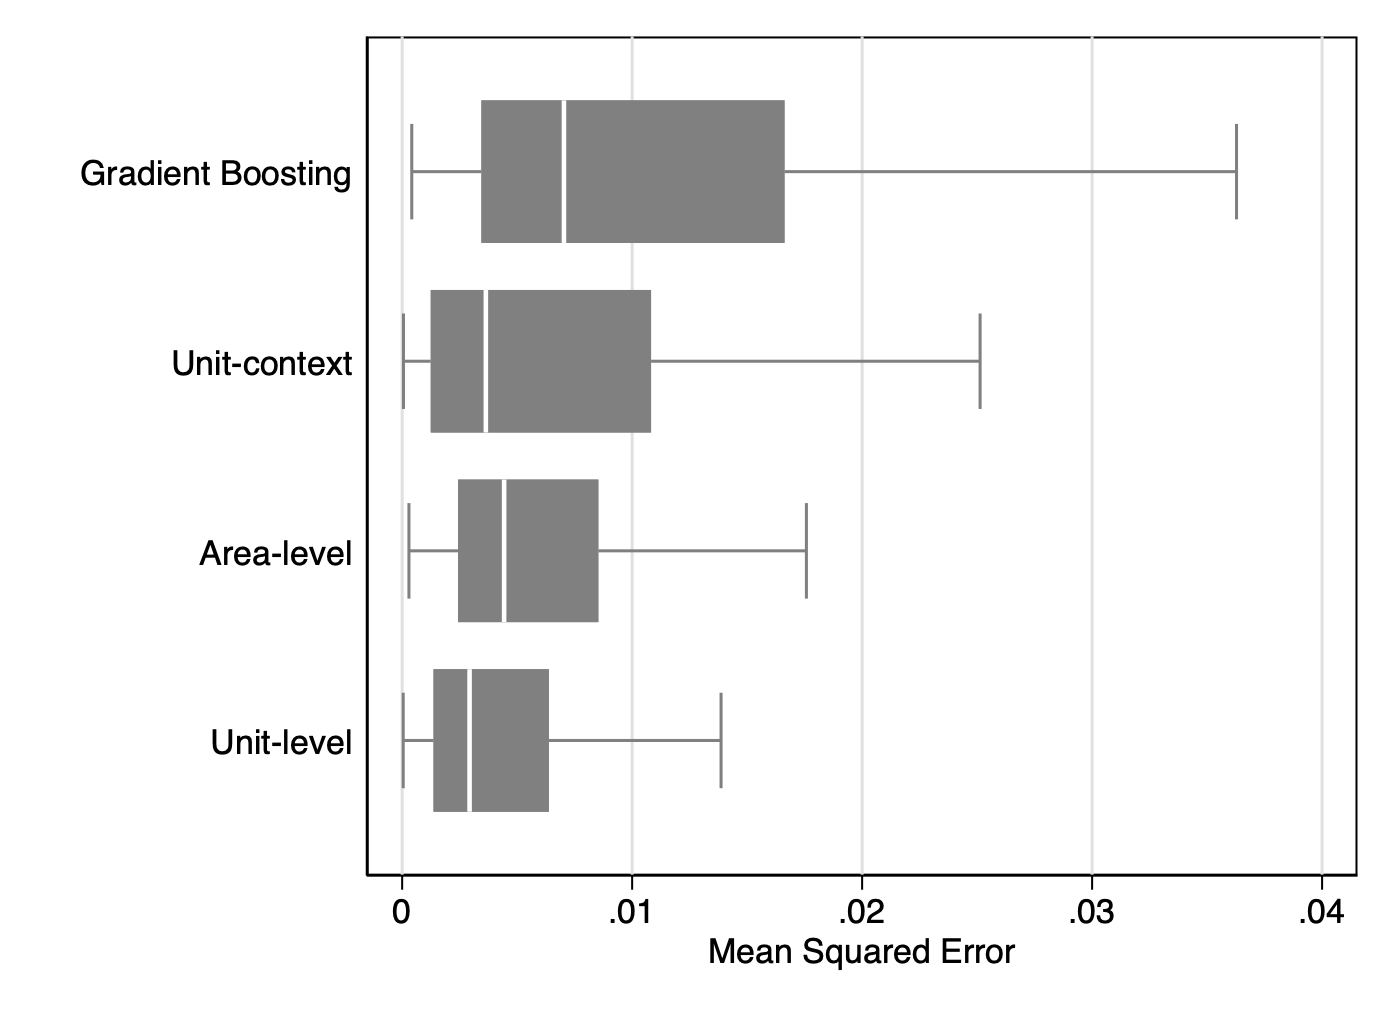
\includegraphics[scale=0.17]{Figure-1a}

}\hfill{}\subfloat[Unconstrained versus constrained]{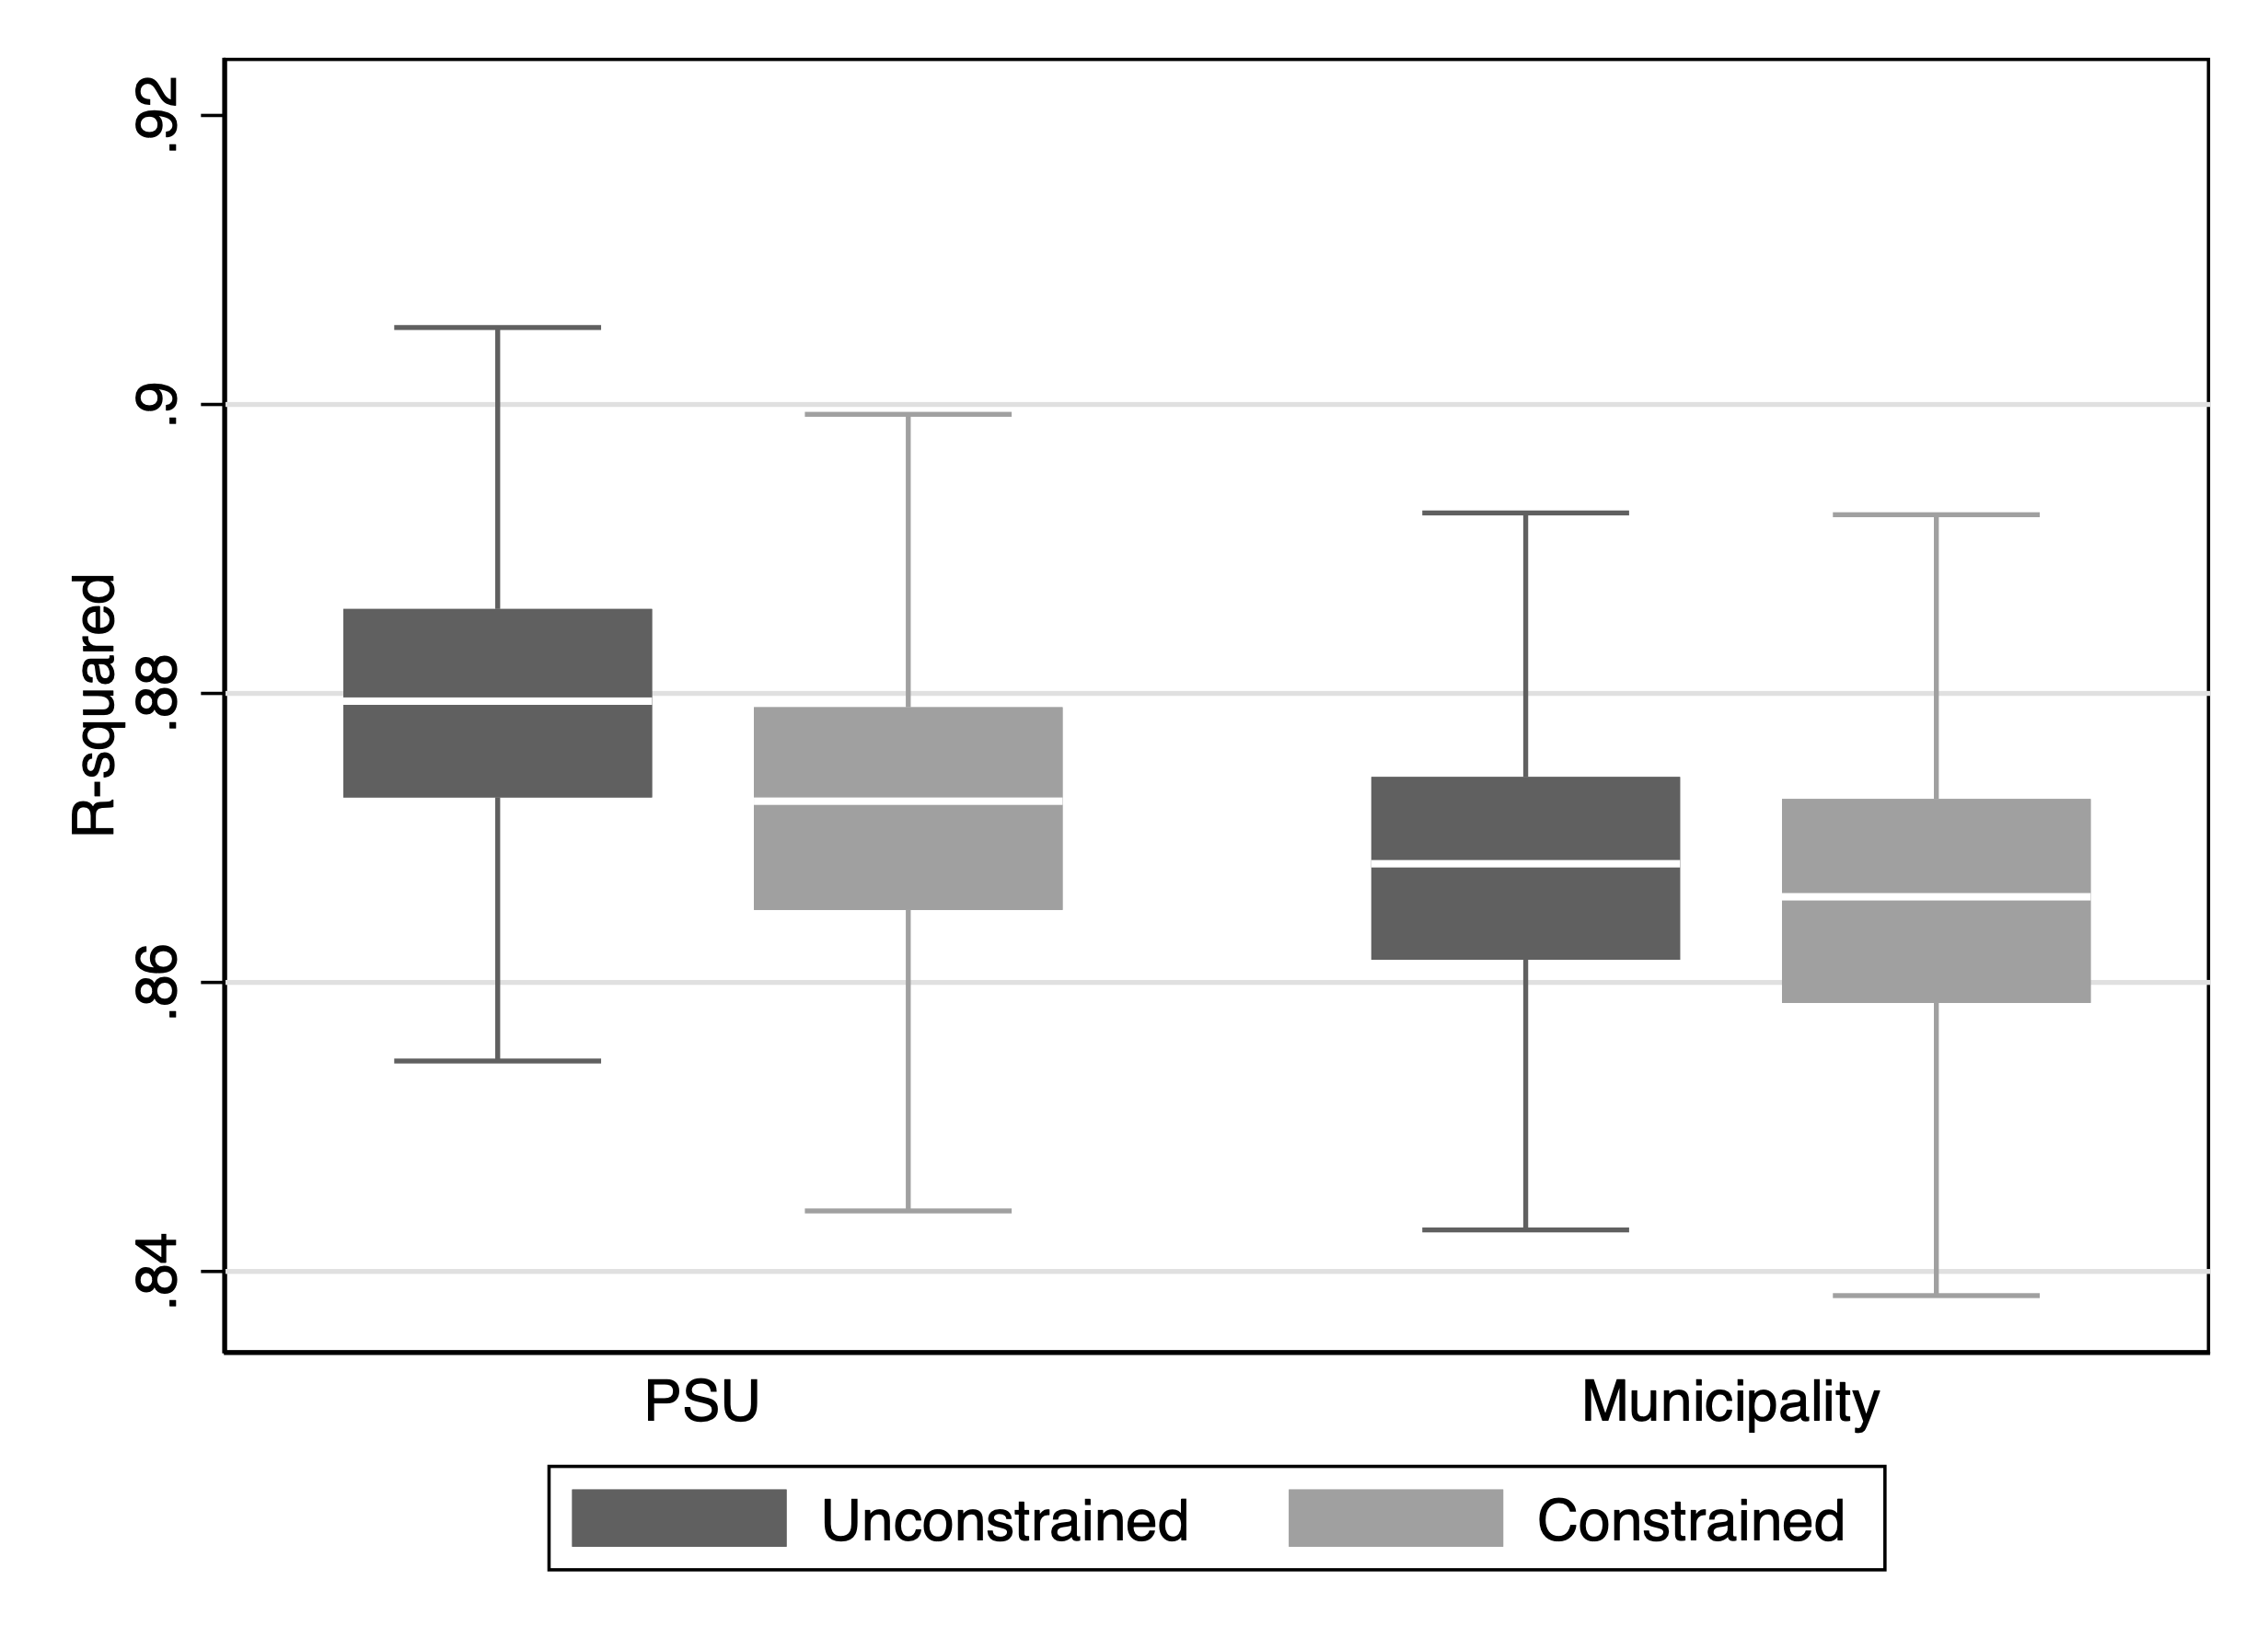
\includegraphics[scale=0.17]{Figure-1b}

}

\caption{$R^{2}$ estimates at the PSU and municipality levels \protect\label{fig:r2}}

\end{figure}

Panel (a) of Figure \ref{fig:r2} presents these results and we find
evidence of considerable downward bias for both the PSU- and municipality-level
models. For example, for the PSU-level model, we find that the median
``true'' $R^{2}$ is 0.88 whereas the median ``direct'' $R^{2}$
is 0.59. Interestingly, the true $R^{2}$ tends to be higher for the
PSU-level model than the municipality-level model, but the opposite
is the case for the direct $R^{2}$. This suggests that model selection
based on the direct $R^{2}$ can be misleading in that the direct
$R^{2}$ incorrectly suggests that the municipality is the preferred
level of estimation. More specifically, we find that the true $R^{2}$
identifies the PSU as the preferred level of estimation for 437 of
the 500 samples, but the direct $R^{2}$ only selects the PSU level
for four of the 500 samples. The direct $R^{2}$ then identifies the
incorrect level of estimation for 433 of the 500 samples. 

In Section \ref{sec:validation}, we discussed two other ways that
the $R^{2}$ can be misleading for assessing model performance: it
is invariant to locational shifts and influenced by the variance of
the true poverty rates. Using the Mexican data, we can assess the
relevance of the former issue by comparing the true $R^{2}$ to a
constrained version of the true $R^{2}$ that fixes the intercept
and coefficient to zero and one, respectively. By constraining the
$R^{2}$ in this manner, we remove its ability to adjust for systematic
differences between the poverty estimates and the true poverty rates.
Panel (b) of Figure \ref{fig:r2} presents the results and we see
that, as expected, the unconstrained $R^{2}$ overstates the model's
performance, albeit only to a small degree. We nevertheless find that
even these small differences can lead to model selection issues. In
particular, the constrained $R^{2}$ identifies the PSU level as the
appropriate level of estimation for 355 of the 500 samples whereas
the unconstrained version, as mentioned, selects the PSU level for
437 out of the 500 samples. The commonly used unconstrained $R^{2}$
then selects the incorrect model for 82 of the 500 samples.

\begin{figure}
\begin{centering}
\subfloat[Mean squared error]{\begin{centering}
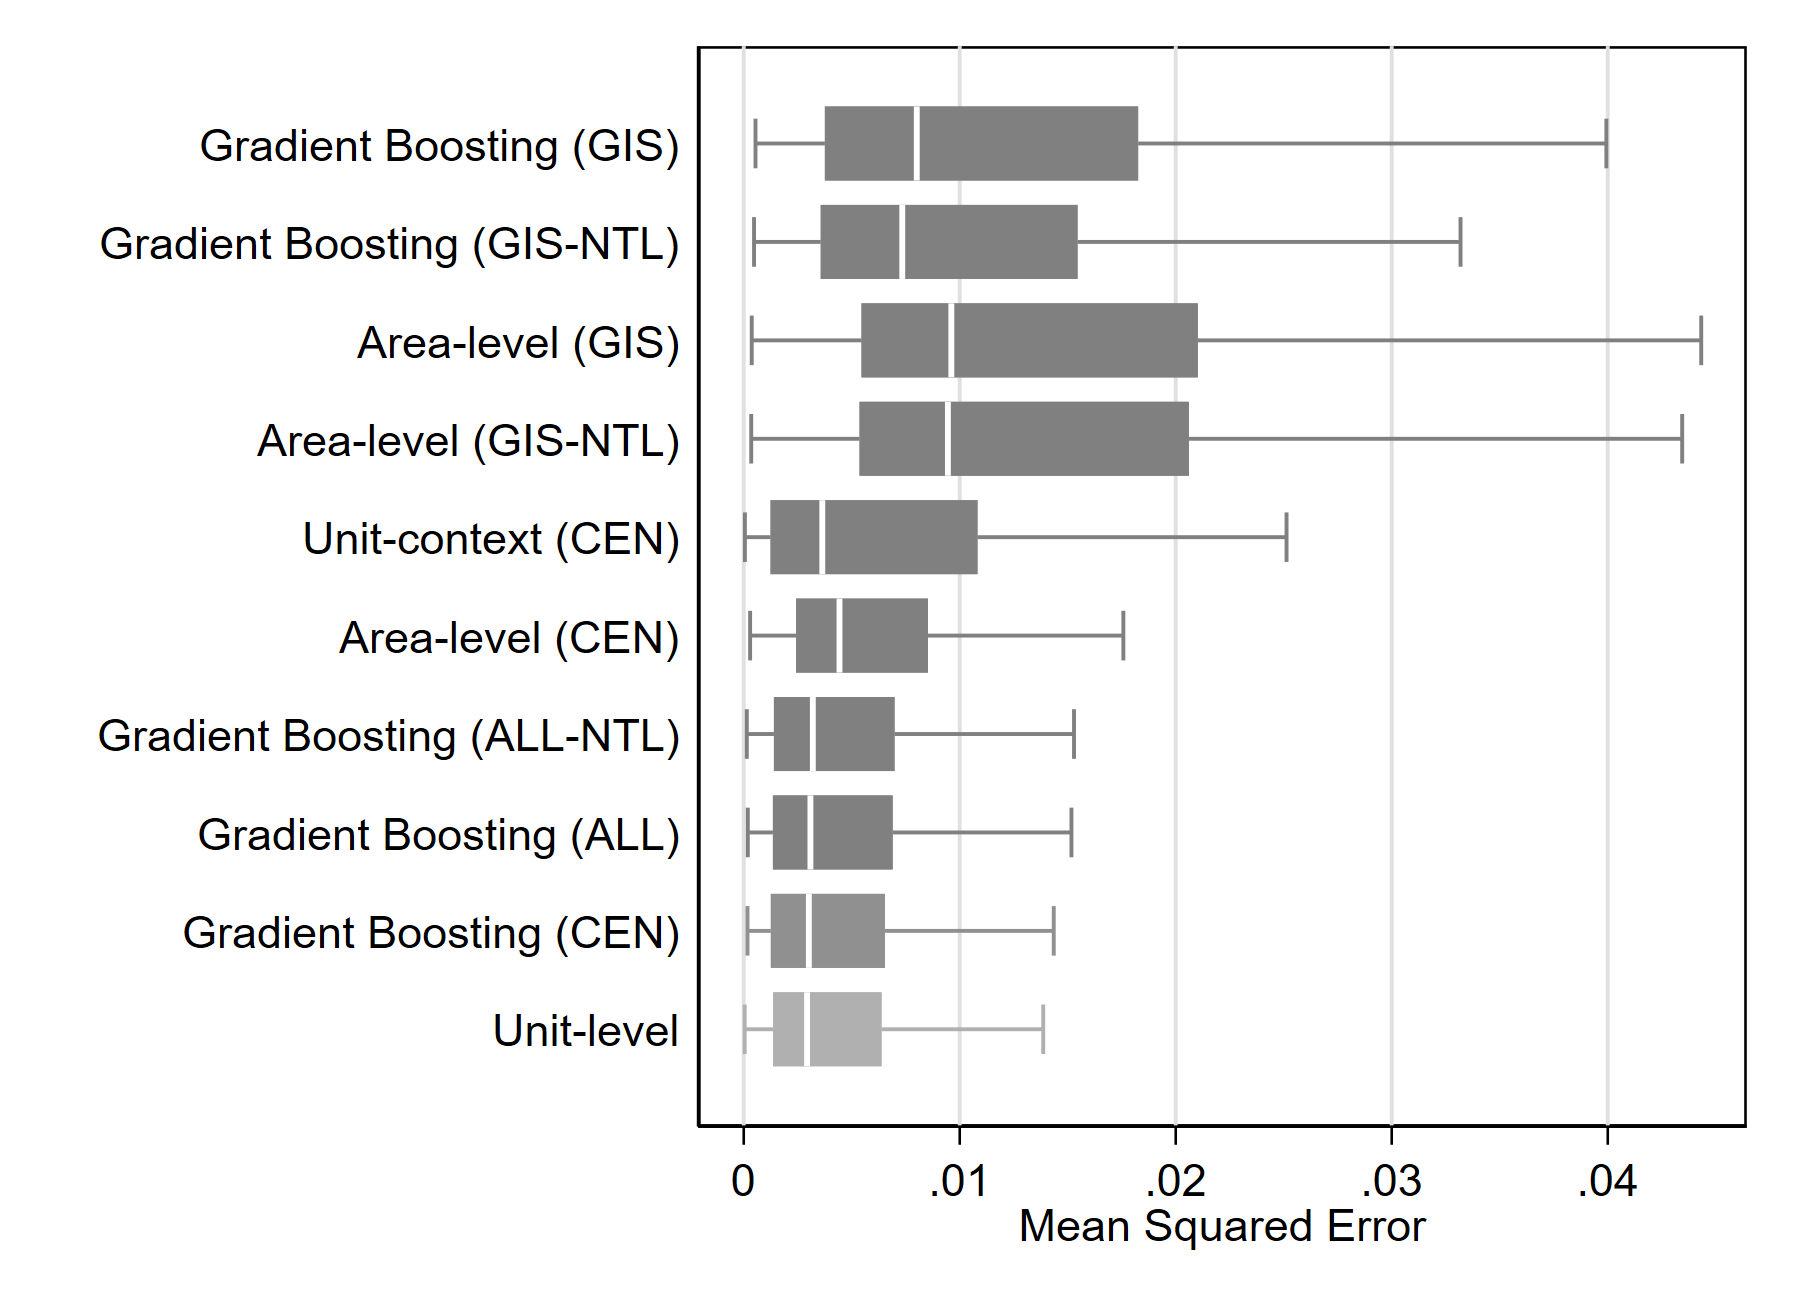
\includegraphics[scale=0.17]{Figure-2a}
\par\end{centering}
}\hspace{0cm}\subfloat[Bias]{\begin{centering}
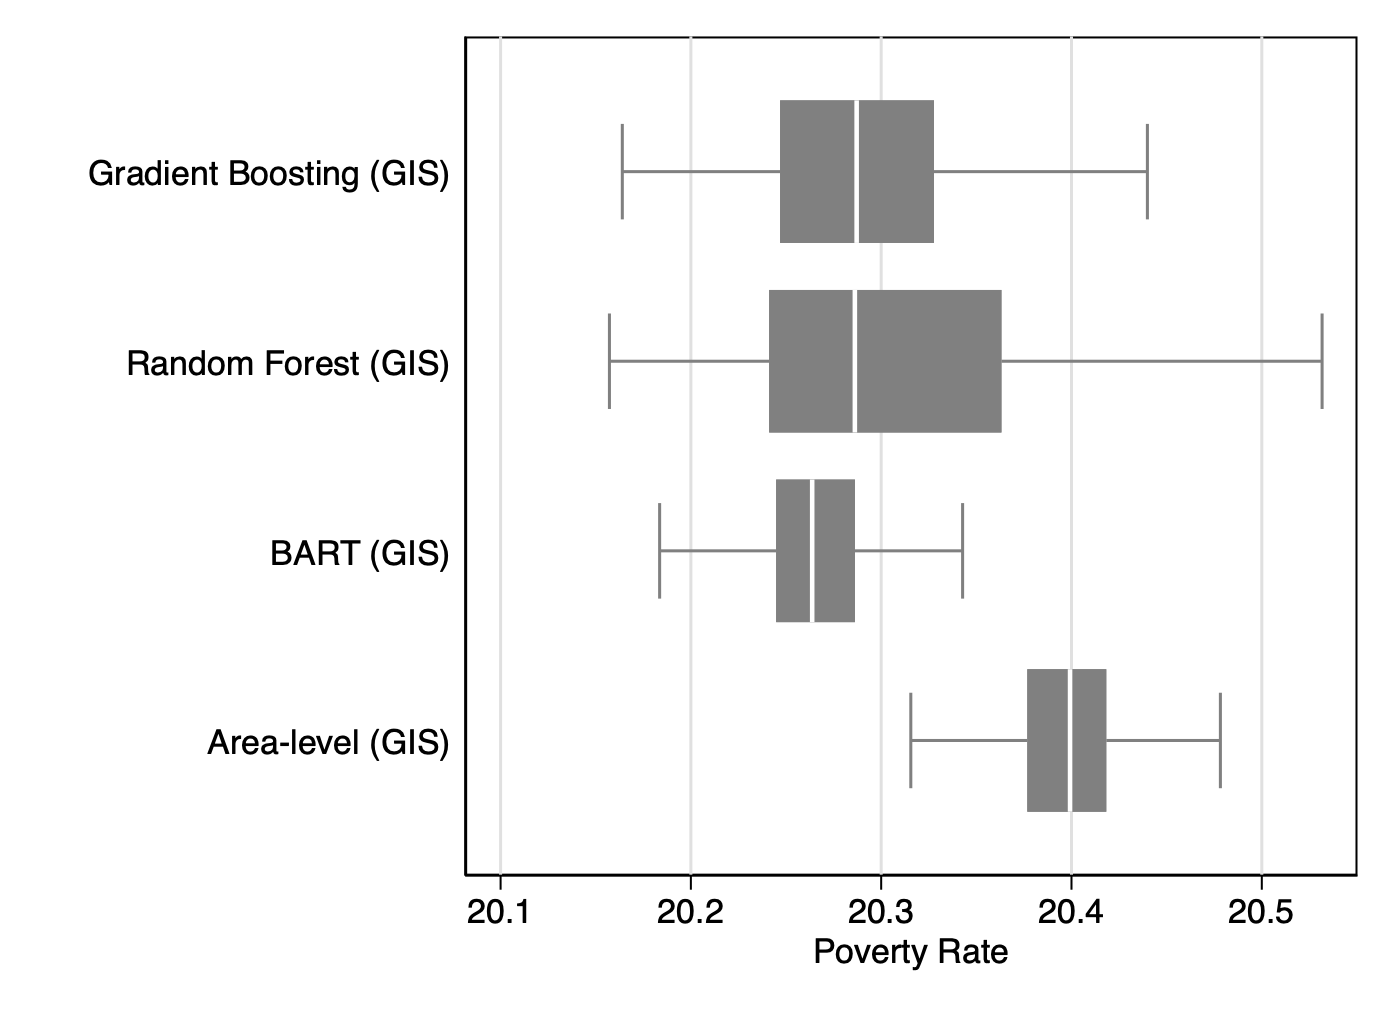
\includegraphics[scale=0.17]{Figure-2b}
\par\end{centering}
}
\par\end{centering}
\centering{}\caption{Mean squared error and bias for select models \protect\label{fig:mse}}
\end{figure}

Given the shortcomings of the $R^{2}$, we have argued that the MSE
represents a better metric for model assessment. Panel (a) of Figure
\ref{fig:mse} thus presents our MSE results for several alternative
models. The first three models apply gradient boosting at the municipality
level using three alternative covariate sets: geo-referenced covariates
(``GIS-MUN''), census-based covariates (``CEN-MUN''), and then
a model with all available covariates (``ALL-MUN''). The fourth
model applies gradient boosting at the PSU level and only uses census-based
covariates (``CEN-PSU'').\footnote{Recall that the geo-referenced covariates are only available at the
municipality level.} The final three models are all traditional methods that we use to
benchmark the performance of gradient boosting. In particular, we
present the unit-level (obtained with CensusEB methods), unit-context
(obtained with CensusEB methods), and area-level models. We consider
three alternative implementations of the area-level model that, much
like for gradient boosting, vary the level of analysis and the covariates
used. For these traditional models, all available covariates enter
the models linearly (i.e., we do not include interaction or quadratic
terms).

One advantage of the MSE is that it can be calculated for each geographical
entity. As such, each box plot in panel (a) of Figure \ref{fig:mse}
summarizes the distribution of municipality-level MSE estimates rather
than the aggregate MSE for each sample (i.e., the results are based
on Eq. {[}\ref{eq:mseg}{]}). It is useful to first consider how gradient
boosting performs relative to the traditional models when using the
same census-based covariates. In this case, the gradient boosting
implementations at the municipality and PSU levels achieve median
MSE values of 0.003 and 0.002, respectively. In contrast, the \textquotedblleft gold
standard\textquotedblright{} unit-level model achieves a median MSE
of 0.003. The remaining traditional methods that use census-based
covariates all achieve a median MSE of roughly 0.004. These results
suggest that, when using the same data, gradient boosting performs
comparably (if not better) than the unit-level model and better than
the unit-context and area-level models. Given that traditional small
area methods tend to make more use of the data at hand, the performance
of gradient boosting is somewhat surprising. It may be due to the
fact that gradient boosting accommodates more flexible functional
forms or it may be something specific to the data at hand.

Recall, however, that the machine-learning approach to poverty mapping
most commonly uses remotely-sensed covariates rather than census-based
covariates. The gradient boosting model with geo-referenced covariates
(``GIS-MUN'') is our closest approximation to this standard implementation.
This model achieves a median MSE of 0.008 (with a root MSE of about
0.09), meaning that the median municipality's error is roughly nine
percentage points. It is useful to compare these results to those
from the unit-context and area-level models given that these models
are direct competitors to machine learning. The unit-context model
and the area-level models with census covariates all achieve median
MSE values of 0.004, whereas the area-level model using geo-referenced
covariates achieves a median MSE of 0.01. With the exception of the
area-level model based on geo-referenced covariates, we thus find
that the standard implementation performs considerably worse than
the traditional methods that are also feasible in off-census years.

The bias associated with poverty estimates is especially important
due to the policy relevance of understanding absolute living standards.
In panel (b) of Figure \ref{fig:mse}, we thus present box plots for
the municipality-level bias estimates associated with each model (see
Eq. {[}\ref{eq:mseg}{]} for the bias-variance decomposition of the
MSE). The median bias for all models is approximately zero, with the
possible exception of the unit-context model and the area-level model
estimated at the PSU level.\footnote{The same issue for unit-context models is highlighted by \citet{corral2021map}
and \citet{corral2022guidelines}.} Perhaps the more interesting result is that the bias estimates from
the gradient boosting model with geo-referenced covariates exhibits
considerable variation, with minimum and maximum biases reaching -0.43
and 0.43, respectively. That is, the standard implementation with
remotely-sensed covariates is severely biased for some municipalities,
even though its median bias is approximately zero. All other models,
including the competing unit-context and area-level models, exhibit
much less variation.

\begin{figure}
\begin{centering}
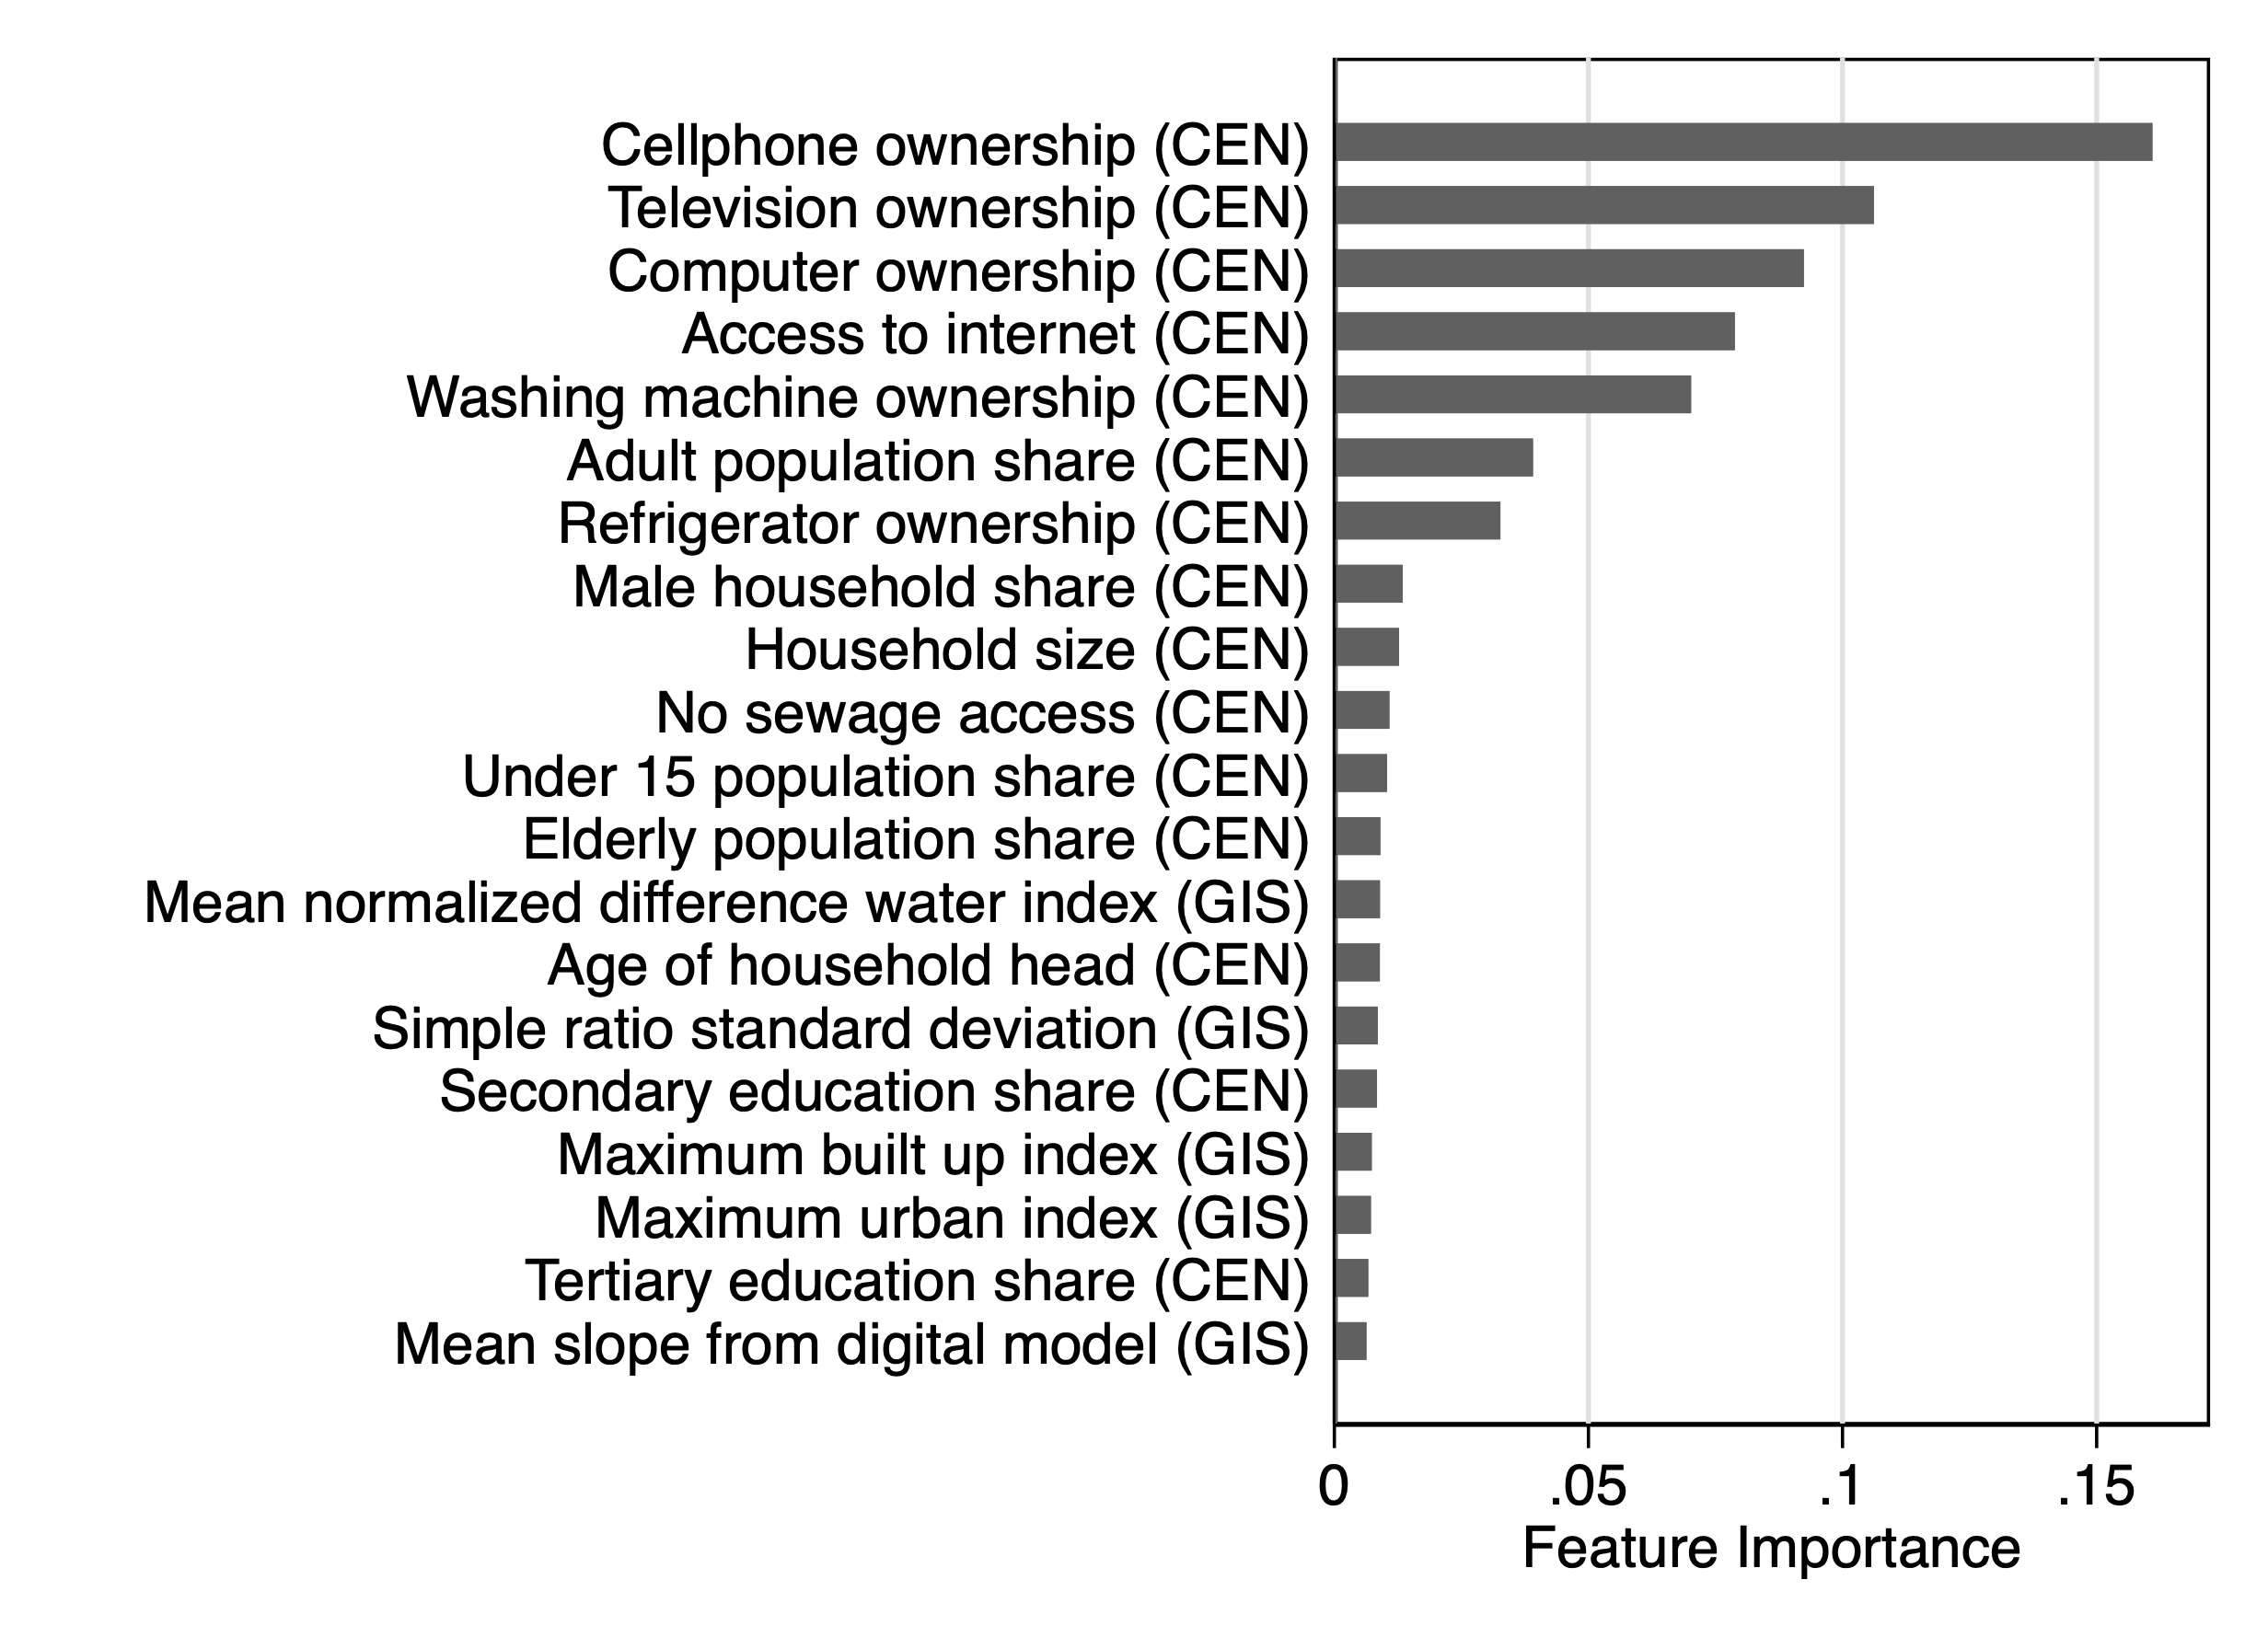
\includegraphics[scale=0.25]{Figure-3.png}
\par\end{centering}
\centering{}\caption{Feature importance\protect\label{fig:importance}}
\end{figure}

The performance of machine learning appears to depend heavily on the
covariates used in the model, with census-based covariates considerably
improving model performance. Another way to see that the census-based
covariates have greater predictive power than the remotely-sensed
covariates is by looking at feature importance. One popular measure
of feature importance summarizes the gain (i.e., reduction of the
loss function) associated with any given feature. That is, for a given
run of the model, feature importance captures the average gain of
a given feature, where the gains are averaged across all trees in
the model.\footnote{In addition, the average gains for a given run of the model are normalized
by dividing each by the sum of all average gains for that run.} Figure \ref{fig:importance} plots the 20 covariates with the highest
feature importance after running gradient boosting with all covariates
on each sample and averaging each covariate's importance across the
500 samples. We find that all of the top 10 covariates are census-based,
with only five geo-referenced covariates entering the top 20.

\begin{figure}
\begin{centering}
\subfloat[Mean squared error]{\begin{centering}
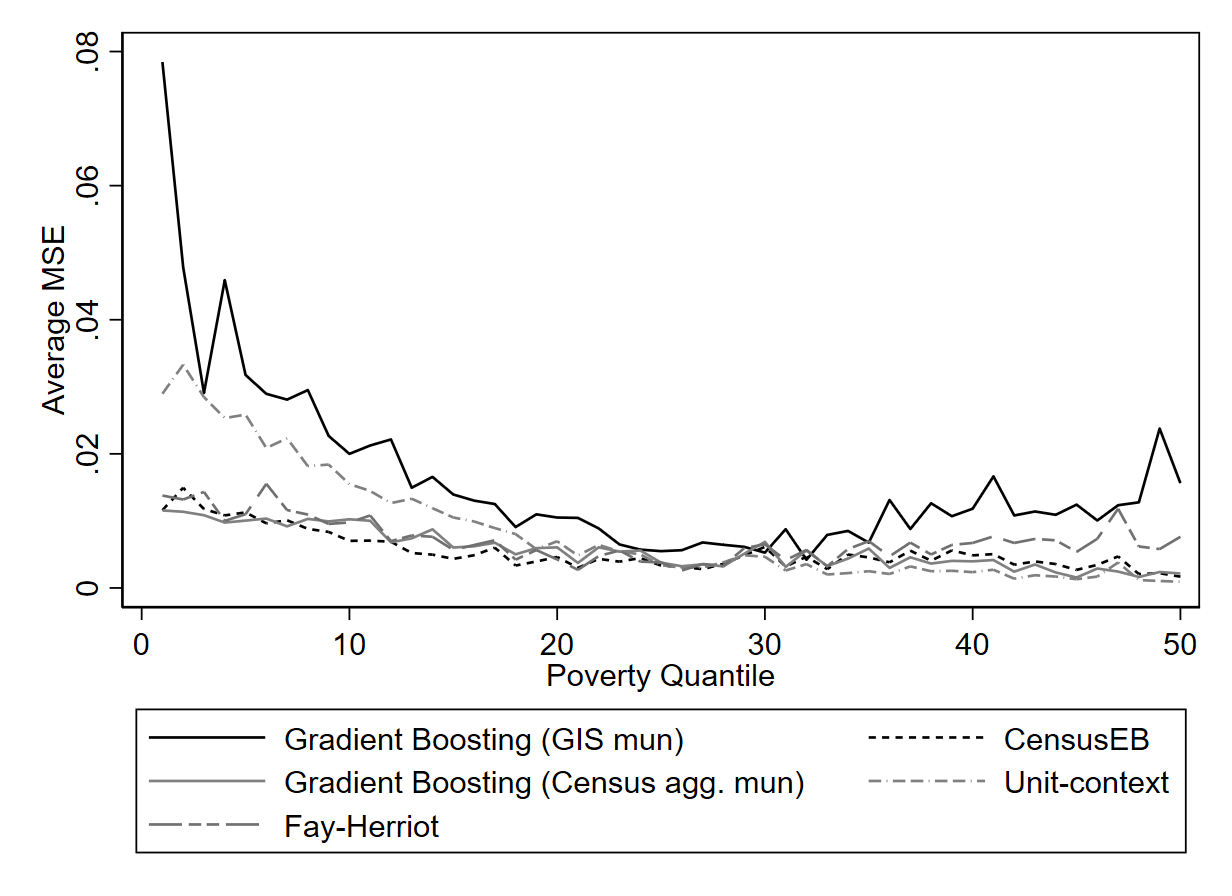
\includegraphics[scale=0.17]{Figure-4a.png}
\par\end{centering}
}\hspace{0cm}\subfloat[Bias]{\begin{centering}
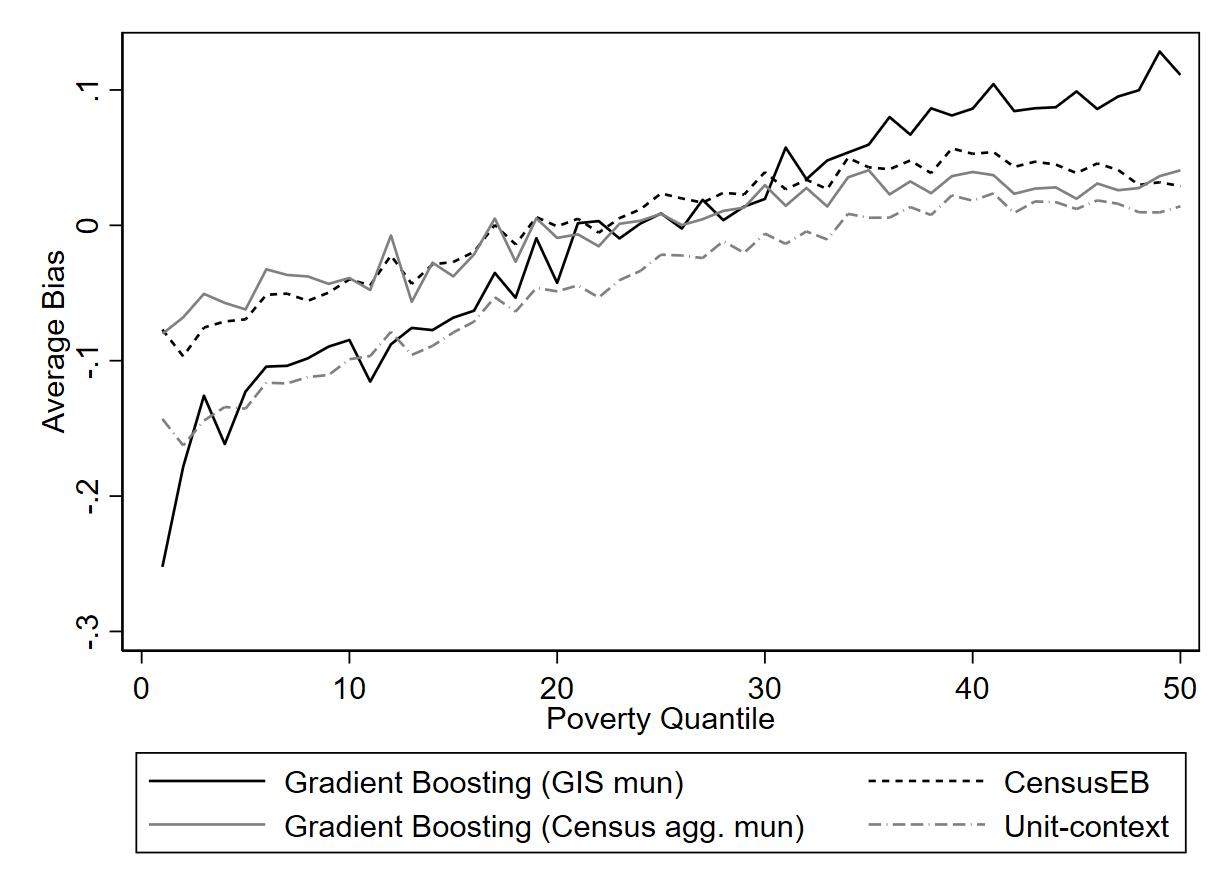
\includegraphics[scale=0.17]{Figure-4b.png}
\par\end{centering}
}
\par\end{centering}
\caption{Mean squared error and bias by poverty quantiles for select models
\protect\label{fig:quantiles}}
\end{figure}

Figure \ref{fig:quantiles} presents MSE and bias estimates for various
models across different ``poverty quantiles.'' That is, we order
all municipalities by their true poverty rates, divide them into 50
quantiles, and calculate the average MSE and bias for each quantile.
For the sake of simplicity, we only present results for two machine-learning
models -- the municipality-level models using only geo-referenced
and census-based covariates -- and select traditional methods. Panel
(a) presents the MSE results and panel (b) presents the bias results.
In both plots, gradient boosting with census-based covariates performs
quite similarly to the ``gold standard'' unit-level model across
all quantiles. However, gradient boosting with geo-referenced covariates
again departs considerably from this benchmark, particularly at the
lowest and highest quantiles. The bias results are particularly notable:
the model with geo-referenced covariates systematically underestimates
poverty at the lowest quantiles and overestimates poverty at the highest
quantiles. The standard implementation thus understates the spatial
distribution of poverty. 

\begin{figure}
\begin{centering}
\subfloat[Design MSE]{\begin{centering}
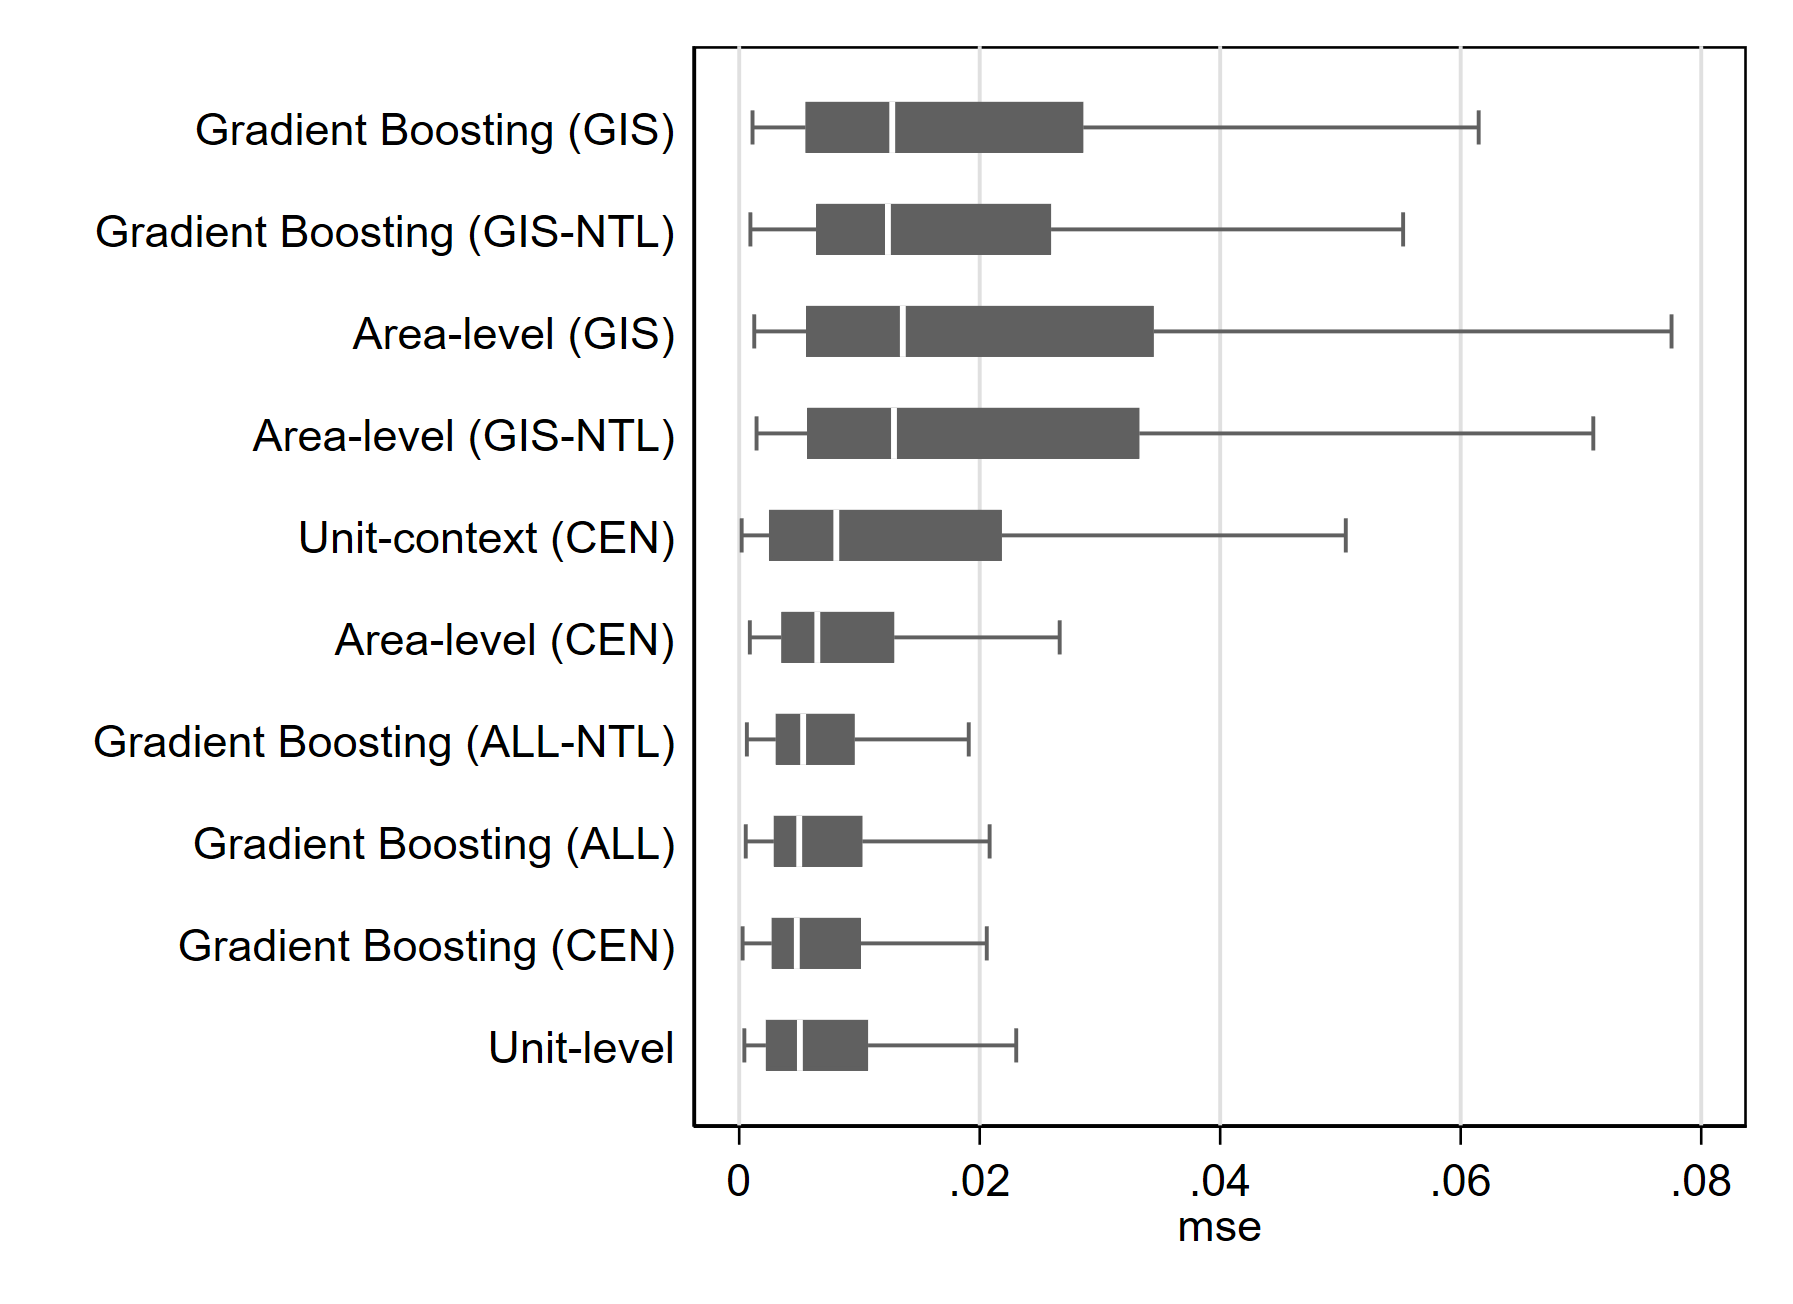
\includegraphics[scale=0.18]{Figure-3_1a.png}
\par\end{centering}
}\hspace{0cm}\subfloat[Design bias]{\begin{centering}
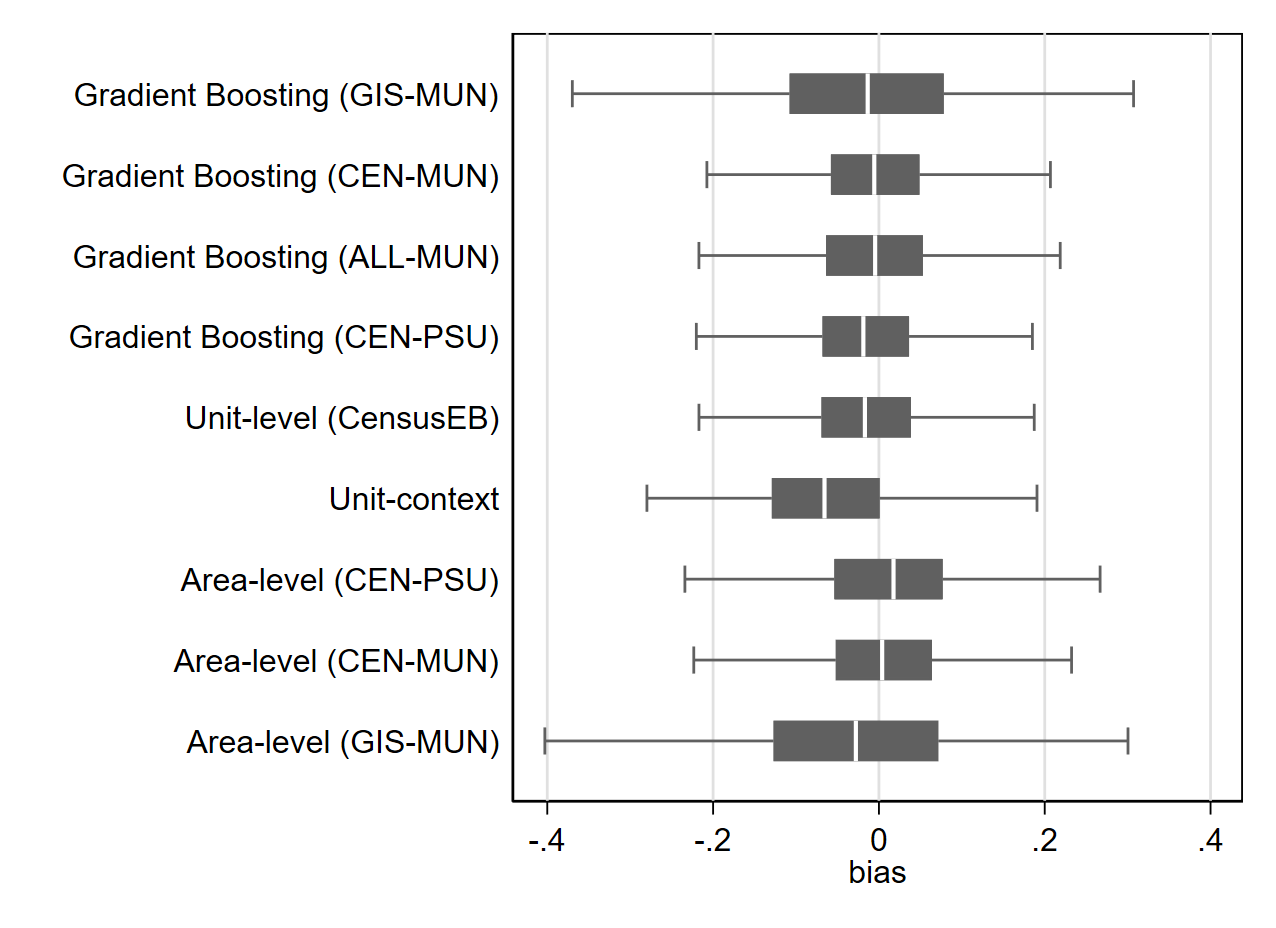
\includegraphics[scale=0.18]{Figure-3_2a.png}
\par\end{centering}
}
\par\end{centering}
\caption{Empirical design MSE and bias with alternative machine-learning models
among 20 percent least likely to be sampled municipalities \protect\label{fig:ll_sample_q1}}
\end{figure}

\begin{figure}
\caption{Empirical design MSE and bias with alternative machine-learning models
among 20 percent most likely to be sampled municipalities \protect\label{fig:ll_sample_q5}}

\centering{}\subfloat[Design MSE]{\begin{centering}
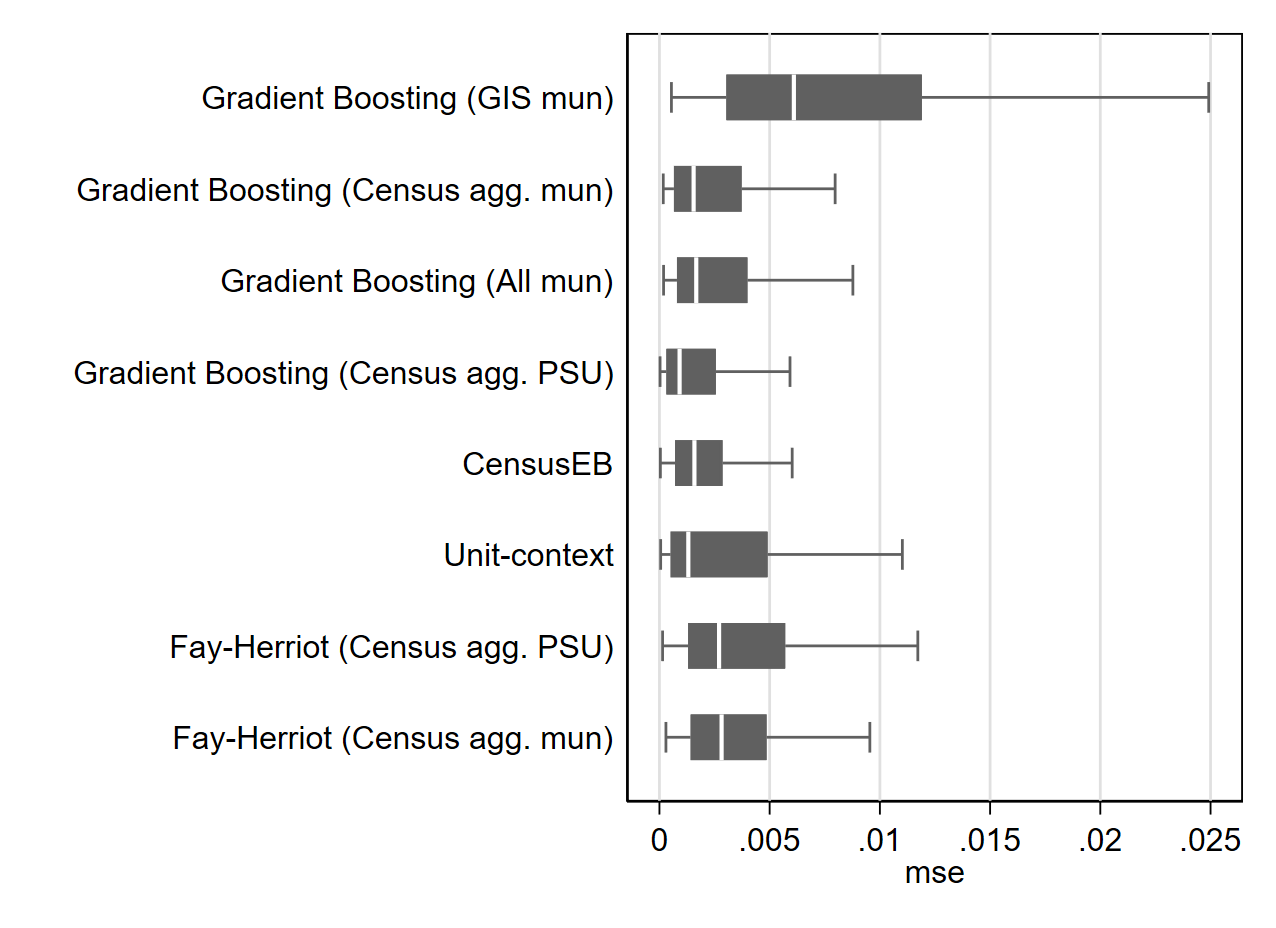
\includegraphics[scale=0.18]{Figure-3_1b.png}
\par\end{centering}
}\hspace{0cm}\subfloat[Design bias]{\begin{centering}
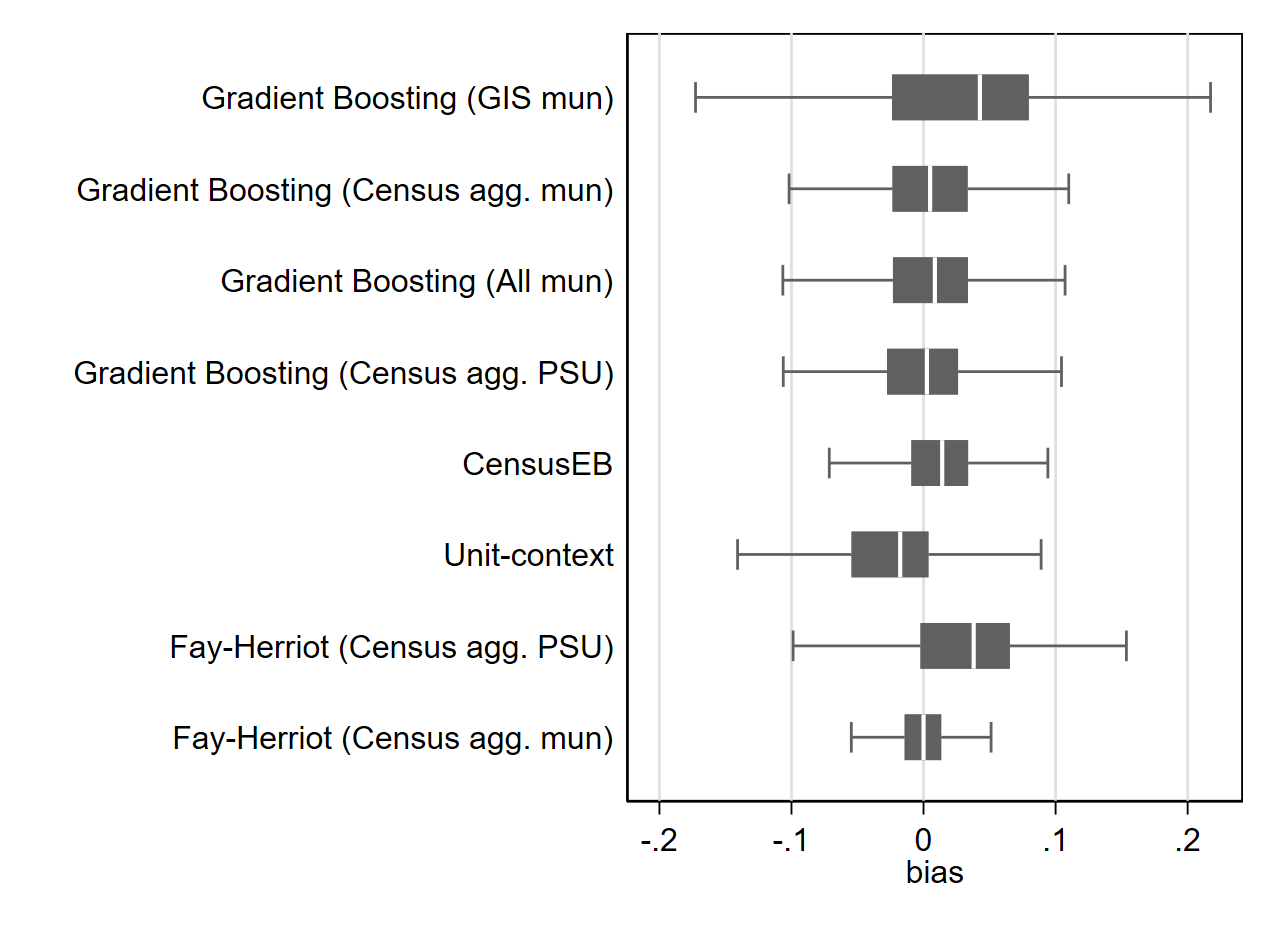
\includegraphics[scale=0.18]{Figure-3_2b.png}
\par\end{centering}
}
\end{figure}

An additional consideration is how the methods perform for predictions
which are out of sample. Because the experiment consists of 500 samples
taken from the census data, a given municipality may be present in
one of the samples and may be absent in others. Consequently, to evaluate
out of sample properties we rank municipalities by their likelihood
of selection across the 500 samples. The likelihood of being present
ranges from 0.09 to 1, with a median of 0.48 and a mean of 0.53. Among
the 20 percent least likely to be sampled municipalities, the gradient
boosting model with GIS-based covariates is the worst performing in
terms of MSE followed closely by unit-context models (Figure \ref{fig:ll_sample_q1}).
In terms of bias among the 20 percent of municipalities that are least
likely to be sampled, the gradient boosting model with the geo-referenced
covariates shows very wide variability, while unit context models
show downward bias. The other gradient boosting models perform similarly
to unit-level models in terms of bias and MSE. The performance, in
terms of MSE, of the different methods seems to improve with the likelihood
of being selected. Among municipalities most likely to be selected,
the gradient boosting model with the geo-referenced covariates is
still the worst performing (Figure \ref{fig:ll_sample_q5}). However,
in terms of bias, among the most likely to be selected municipalities,
the bias of Fay-Herriot methods at the municipality level is the best
performing illustrating the importance of the method's EBLUP.

\begin{figure}
\begin{centering}
\subfloat[Mean squared error]{\begin{centering}
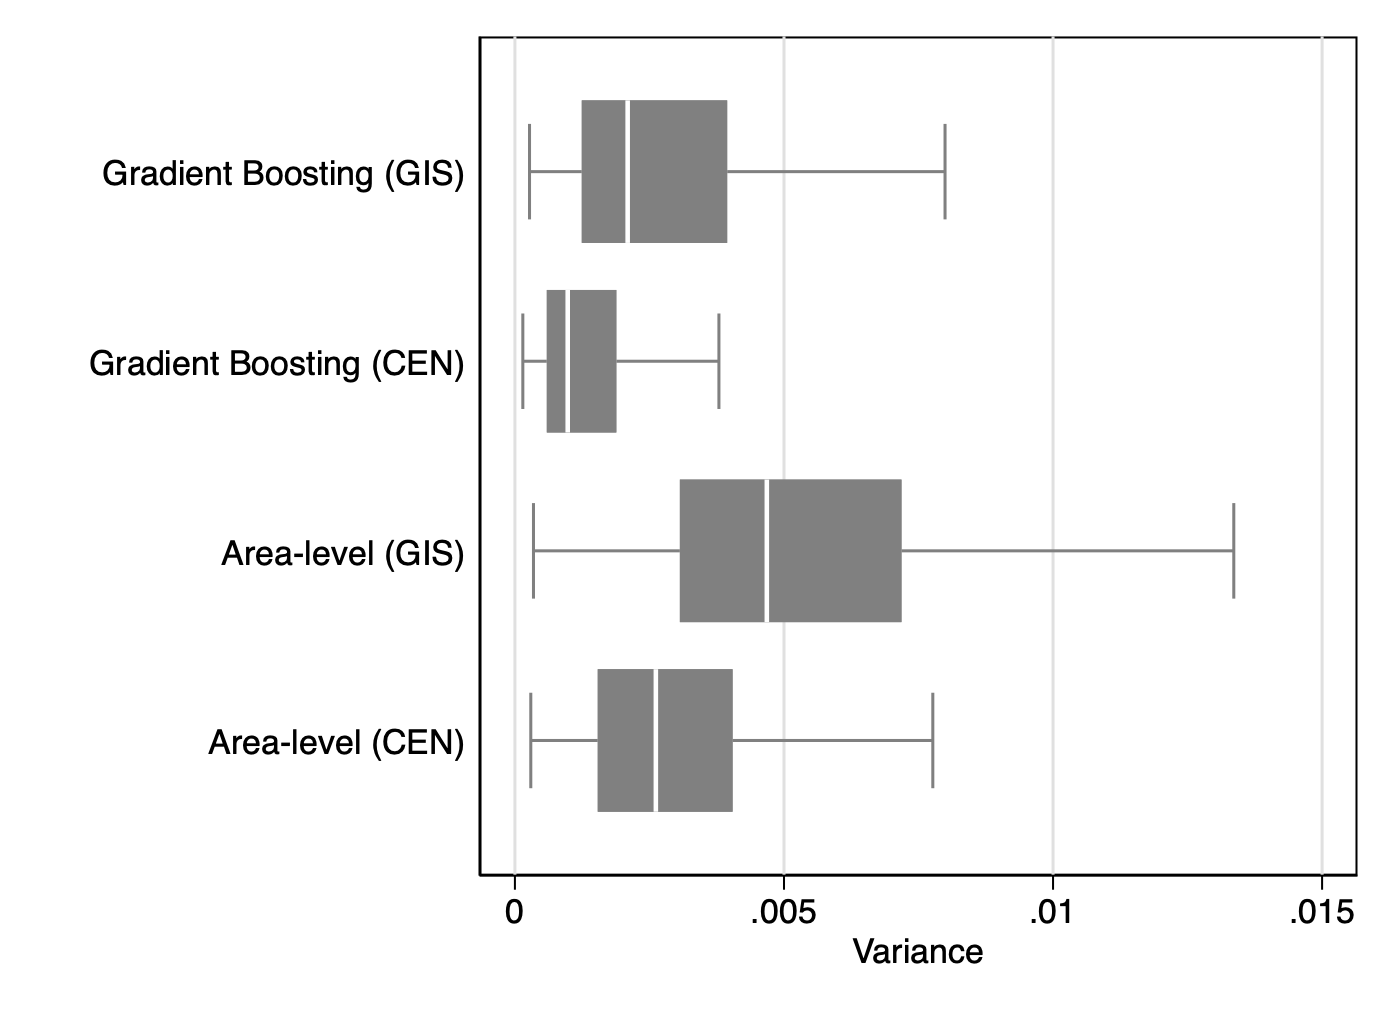
\includegraphics[scale=0.17]{Figure-5a}
\par\end{centering}

}\hspace{0cm}\subfloat[Bias]{\begin{centering}
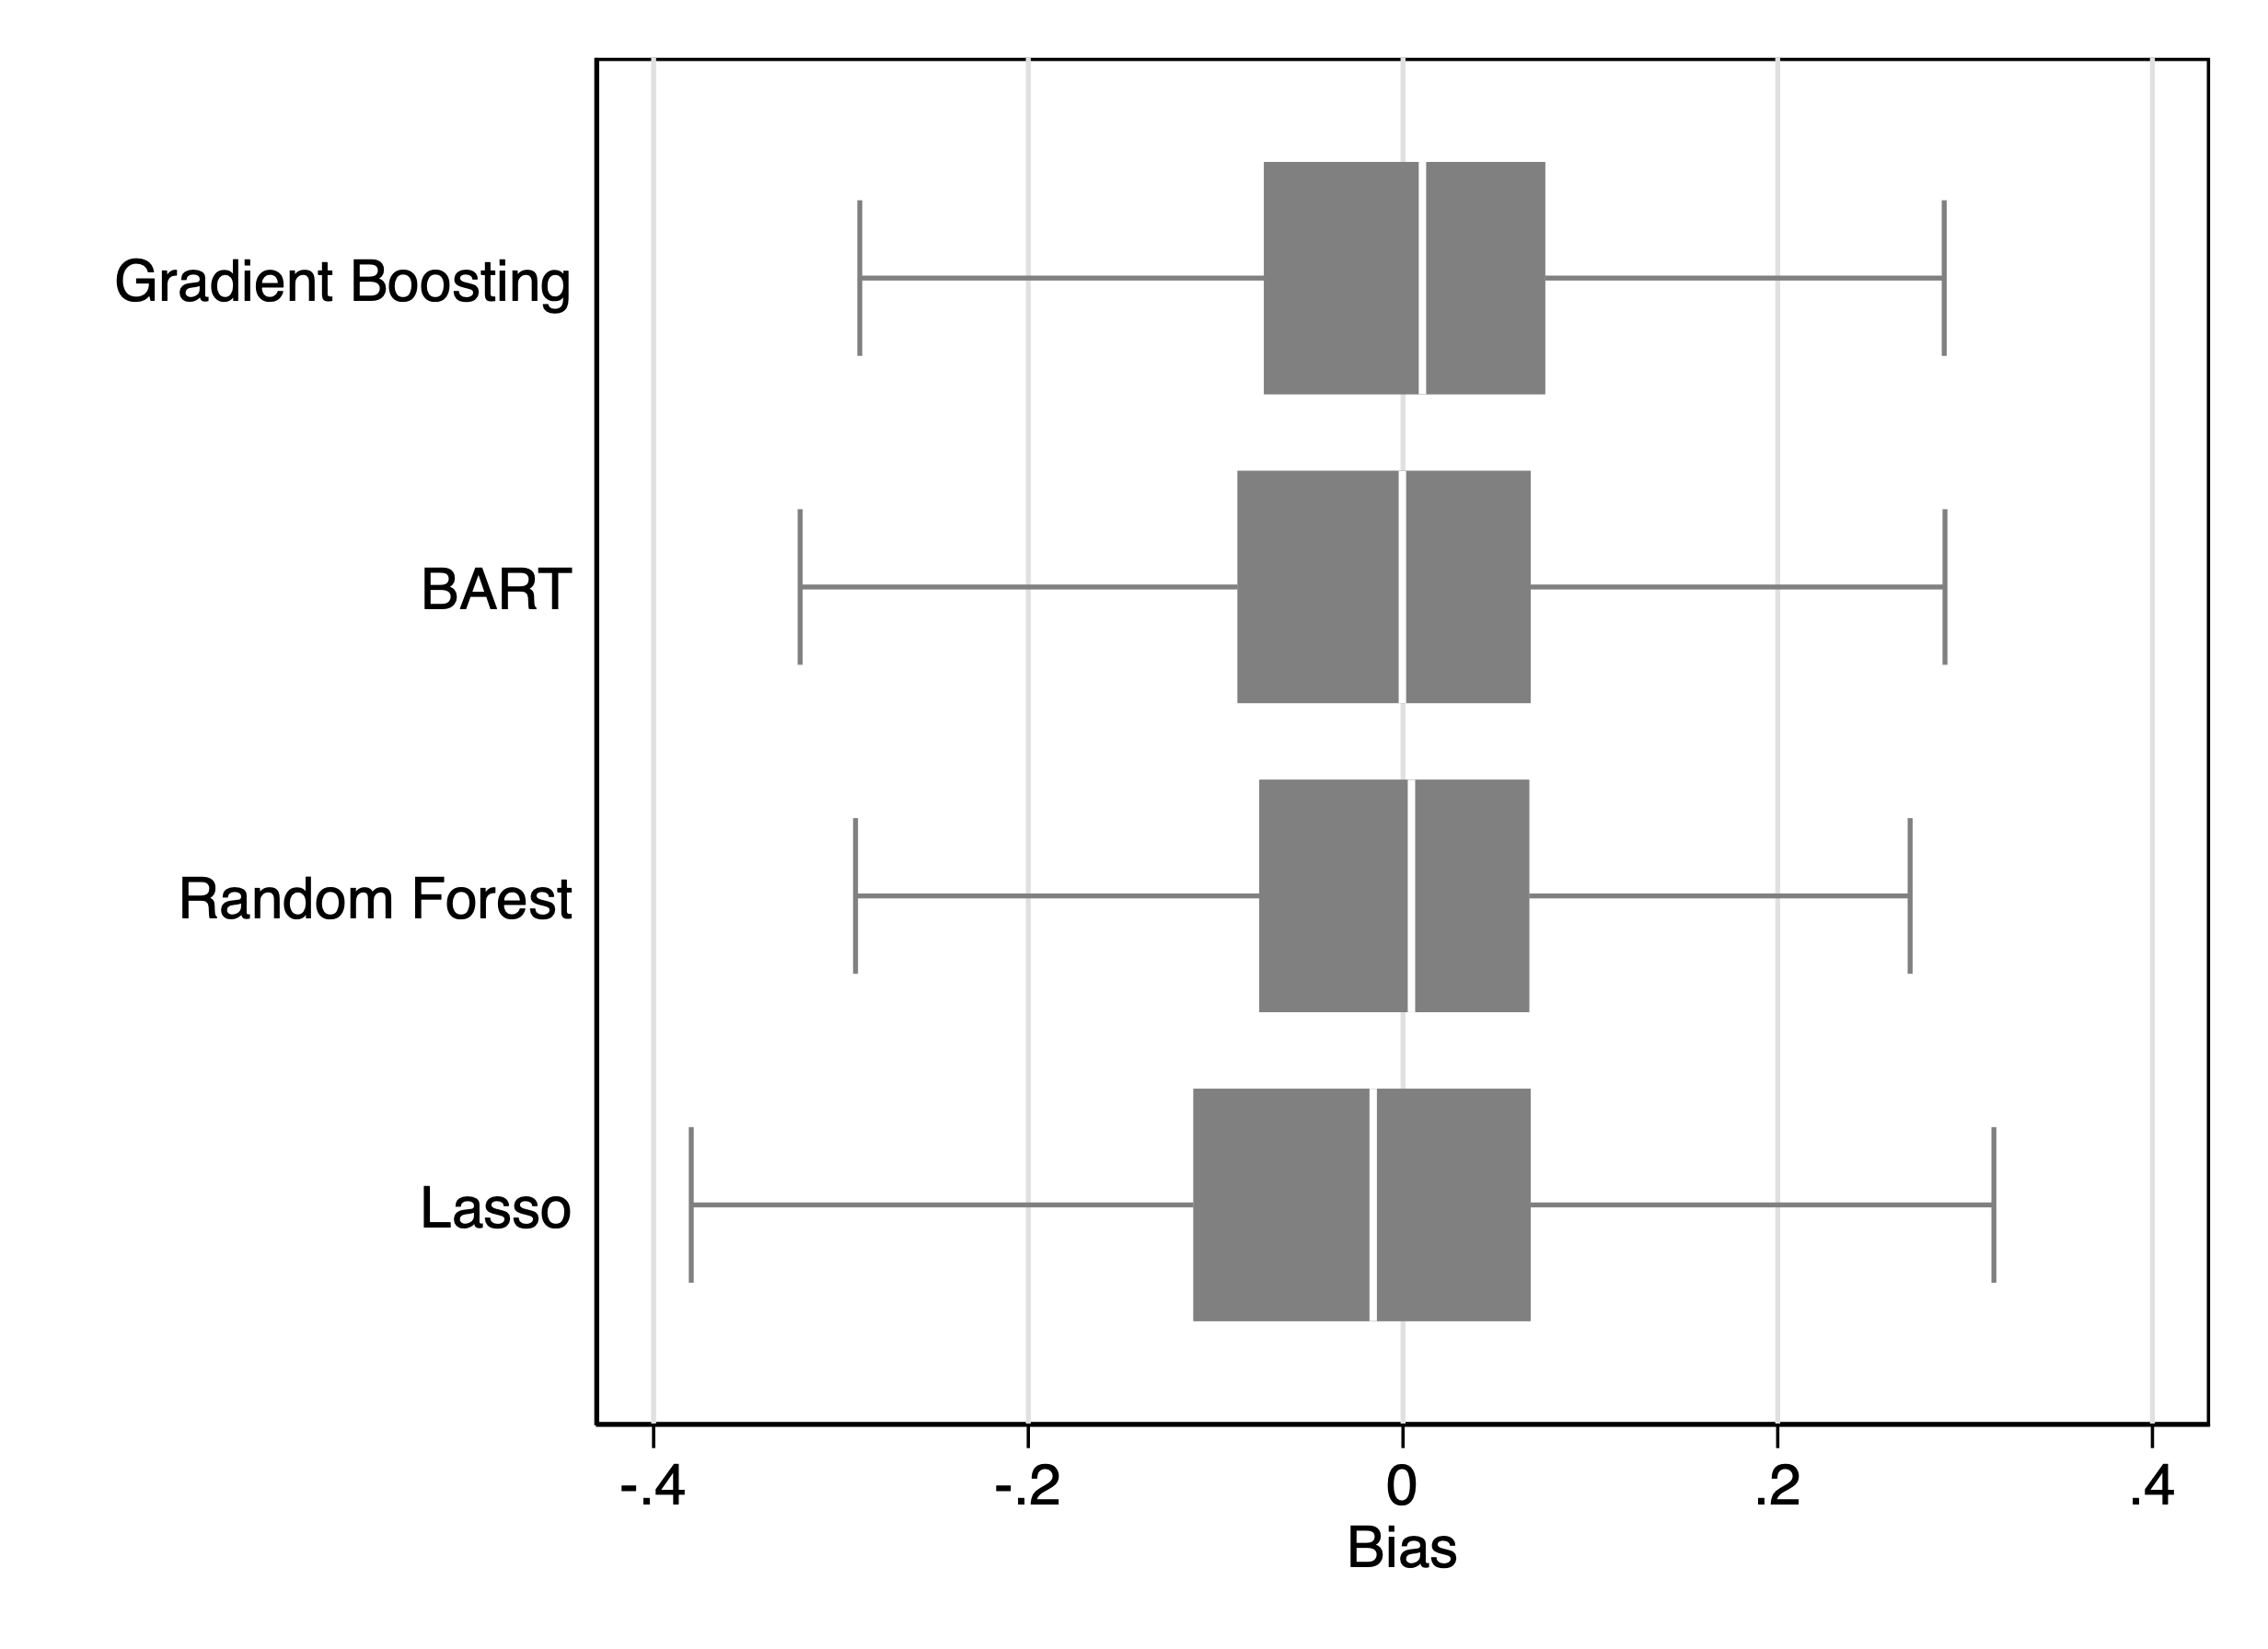
\includegraphics[scale=0.17]{Figure-5b}
\par\end{centering}

}
\par\end{centering}
\caption{Mean squared error and bias for alternative machine learning models
\protect\label{fig:ml}}
\end{figure}

While we have focused on the performance of gradient boosting up to
this point, there are nevertheless several other machine-learning
models that can be used for poverty mapping. Leading alternatives
include the least absolute shrinkage and selection operator (lasso)
\citep{tibshirani1996}, the random forest \citep{breiman2001}, and
Bayesian additive regression trees (BART) \citep{chipman2010bart}.
While the lasso is a simple way to conduct variable selection and
regularization in the context of linear regression, the random forest
and BART models are similar to gradient boosting in that they all
rely on regression tree frameworks. We ask whether these alternative
models can perform better than gradient boosting within the confines
of the standard implementation, which relies exclusively on remotely-sensed
covariates. Panels (a) and (b) of Figure \ref{fig:ml} present the
MSE and bias results for all models. With the possible exception of
the lasso, we find that all models perform comparably, meaning that
the performance of gradient boosting when using geo-referenced covariates
cannot be remedied by simply adopting a different machine-learning
model.

\begin{figure}
\begin{centering}
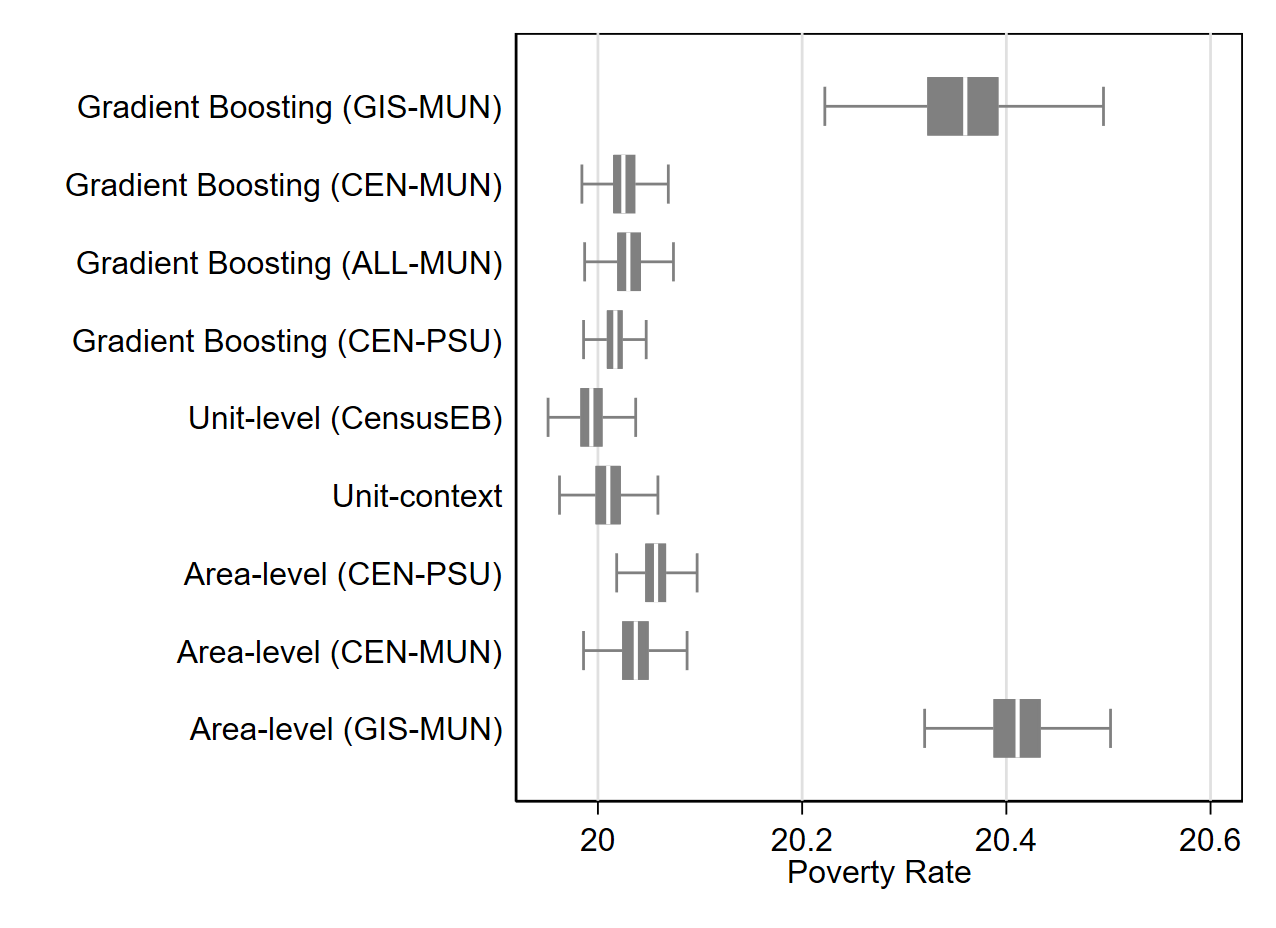
\includegraphics[scale=0.25]{Figure-6.png}
\par\end{centering}
\caption{Poverty targeting \protect\label{fig:targeting}}
\end{figure}

Finally, recall from Section \ref{sec:validation} that we argued
that the ultimate concern with poverty mapping is to understand how
different methodological choices affect poverty alleviation. Figure
\ref{fig:targeting} thus compares the machine-learning and traditional
approaches in terms of their ability to reduce poverty in the context
of our targeting simulations. In these simulations, which is dependent
just on the povertyu ranking, a hypothetical poverty-alleviation program
targeted on the basis of \textit{true} municipality-level poverty
rates is able to reduce the overall poverty headcount to just under
20 percent, a 5 percentage point improvement. While the achieved poverty
rates of all models fall within the 20 percent range, we find that
gradient boosting with geo-referenced covariates is one of the worst
performing models. With the exception of the area-level model using
geo-referenced covariates, the standard gradient boosting implementation
relying on geospatial covariates is thus outperformed by all traditional
methods, including those that are direct competitors. However, when
incorporating census-based covariates, we find that gradient boosting
achieves poverty rates that are comparable to the traditional methods,
yet again showing that an exclusive reliance on remotely-sensed data
can limit the performance of the machine learning. 

The results of the targeting simulation are relevant to cases where
targeting is based solely on the ranking of municipalities -- all
methods appear to do a solid job. Nevertheless, there are many instances
where the targeting mechanism may rely on the method's poverty estimates.
For example, Senegal's Unique National Registry (RNU - in French)
of vulnerable households relies on actual estimates from poverty maps
to determine the quotas for sampling by municipality (Ferre \citeyear{ferresenegal}).
It is in those cases where a method that yields unbiased and precise
estimates should be employed.

\section{Conclusion\protect\label{sec:conclusion}}

Machine-learning approaches to poverty mapping have gained considerable
popularity in recent years. In contrast to traditional poverty mapping
procedures, modern machine-learning methods rely on non-parametric
statistical techniques applied to remotely-sensed data, such as satellite
imagery or call detail records. In addition, machine-learning approaches
generally conduct model assessment using the coefficient of determination
($R^{2}$), which is calculated by regressing direct, survey-based
poverty estimates on model predictions. While direct estimates are
unbiased, they can be imprecise measures of true poverty rates and,
as a result, it is unclear whether this form of assessment is informative
of model performance. In this paper, we thus conducted a more rigorous
assessment of the machine-learning approach to poverty mapping by
using the Mexican Intercensal Survey for several design-based simulation
experiments. 

We first showed analytically that that the $R^{2}$ can be a misleading
measure of model performance: it is biased downward when direct estimates
are used as the reference measure of model performance, it is insensitive
to differences in location and scale between the reference measure
and the model predictions, and it is influenced by the variance of
the reference measure. One practical issue this raises is that it
can be misleading to compare the performance of poverty mapping methods
across different datasets, as is done in \citet{yeh2020using}, \citet{chi2022microestimates},
and \citet{aiken2022machine}, among others. Most notably, survey
design elements can affect measurement error in the direct estimates
(e.g., through different sample sizes), which in turn influences the
magnitude of bias in the $R^{2}$. All else equal, models applied
to low-bias settings will appear to perform better than those applied
to high-bias settings. 

Our simulations built on these analytical results. First, we showed
empirically that the direct $R^{2}$ exhibits considerable downward
bias, with the true $R^{2}$ being roughly 35 to 50 percent higher
than the direct $R^{2}$. We also showed that this bias has implications
for model selection, as the direct $R^{2}$ commonly identified the
incorrect level of estimation in our data. Second, we assessed the
performance of machine learning against true poverty rates and found
that the standard implementation using remotely-sensed covariates
performs relatively poorly in terms of mean squared error and bias.
When using census-based covariates, however, we found that machine
learning performs comparably to several traditional poverty mapping
methods. Finally, in the context of targeting simulations, we similarly
found that the standard implementation exhibits relatively poor performance.
This performance deficit was once again remedied with the use of census-based
covariates.

Our results have several implications for the practice of poverty
mapping. For one, our results suggest caution when using $R^{2}$
as a model assessment tool, especially when it is calculated using
direct poverty estimates as the reference measure. We recommend evaluating
the performance of poverty maps using mean squared error, bias, and
targeting simulations, ideally with true poverty rates as the reference
measure. Perhaps the most interesting implication of our results,
however, is that the use of non-parametric statistical methods does
not appear to improve the accuracy of poverty maps relative to traditional
parametric methods. When using the same data, all methods perform
similarly across all metrics. As a result, we recommend that machine-learning
implementations make better use of census-based covariates rather
than relying exclusively on remotely-sensed data. The machine-learning
algorithm can determine whether the census data is truly outdated
and uninformative.

Finally, it is worth emphasizing the limitations of our analysis.
One issue is that we have only examined the performance of machine
learning in the context of the Mexican Intercensal Survey. Similar
simulations using data from other countries may find different results.
For example, it is possible that the same remotely-sensed covariates
have greater predictive power in countries that are lesser-developed
and more reliant on the primary sector. It is also possible that the
remotely-sensed covariates we use in our implementations have less
predictive power than the remotely-sensed data used in other applications.
For example, many applications have used call detail records to produce
poverty maps, but we did not have access to similar data from Mexico.
A natural avenue for future research is then to conduct similar simulations
using data from other countries, possibly with richer forms of remotely-sensed
data.

\pagebreak{}

\bibliographystyle{apalike}
\bibliography{References}

\end{document}
